%%%%%%%%%%%%%%%%%%%%%%%%%%% asme2ej.tex %%%%%%%%%%%%%%%%%%%%%%%%%%%%%%%
% Template for producing ASME-format journal articles using LaTeX    %
% Written by   Harry H. Cheng, Professor and Director                %
%              Integration Engineering Laboratory                    %
%              Department of Mechanical and Aeronautical Engineering %
%              University of California                              %
%              Davis, CA 95616                                       %
%              Tel: (530) 752-5020 (office)                          %
%                   (530) 752-1028 (lab)                             %
%              Fax: (530) 752-4158                                   %
%              Email: hhcheng@ucdavis.edu                            %
%              WWW:   http://iel.ucdavis.edu/people/cheng.html       %
%              May 7, 1994                                           %
% Modified: February 16, 2001 by Harry H. Cheng                      %
% Modified: January  01, 2003 by Geoffrey R. Shiflett                %
% Use at your own risk, send complaints to /dev/null                 %
%%%%%%%%%%%%%%%%%%%%%%%%%%%%%%%%%%%%%%%%%%%%%%%%%%%%%%%%%%%%%%%%%%%%%%

%%% use twocolumn and 10pt options with the asme2ej format
\documentclass[twocolumn,10pt]{asme2ej}
%%\documentclass[twocolumn,15pt]


\usepackage{epsfig} %% for loading postscript figures
\usepackage{amssymb,amsmath}
\usepackage{amsfonts}
\usepackage{multirow}
%\usepackage{natbib}
\usepackage{relsize}
\usepackage{graphicx}
\usepackage{color}
\usepackage{comment}

\usepackage[T1]{fontenc}


\newtheorem{theorem}{Theorem}[section]
\newtheorem{corollary}{Corollary}
\newtheorem*{main}{Main Theorem}
\newtheorem{lemma}[theorem]{Lemma}
\newtheorem{proposition}{Proposition}
\newtheorem{conjecture}{Conjecture}
\newtheorem*{problem}{Problem}
%\theoremstyle{definition}
\newtheorem{definition}[theorem]{Definition}
\newtheorem{remark}{Remark}
\newtheorem*{notation}{Notation}

\providecommand{\keywords}[1]{\textbf{\textit{Index terms---}} #1}
\newcommand{\uu}{{\bf u}}
\newcommand{\vv}{{\bf v}}
\newcommand{\ww}{{\bf w}}
\newcommand{\WW}{{\bf W}}
\newcommand{\nn}{{\bf n}}
\newcommand{\ttt}{{\bf t}}
\newcommand{\pp}{{\bf p}}
\newcommand{\qq}{{\bf q}}
\newcommand{\aaa}{{\bf a}}
\newcommand{\bbb}{{\bf b}}
\newcommand{\yy}{{\bf y}}
\newcommand{\xx}{{\bf x}}
\newcommand{\OO}{\mathbb{O}}
\newcommand{\II}{\mathbb{I}}
\newcommand{\IR}{\mathbb{R}}
\newcommand{\IZ}{\mathbb{Z}}
\newcommand{\half}{\frac{1}{2}}
\newcommand{\bea}{\begin{eqnarray*}}
\newcommand{\eea}{\end{eqnarray*}}
\newcommand{\bfmu}{\mbox{\boldmath $\mu$ \unboldmath} \hskip -0.05 true in}
\newcommand{\bfphi}{\mbox{\boldmath $\phi$ \unboldmath} \hskip -0.05 true in}
\newcommand{\beq}{\begin{equation}}
\newcommand{\eeq}{\end{equation}}
\newcommand{\bfomega}{\mbox{\boldmath $\omega$ \unboldmath} \hskip -0.05 true in}
\newcommand{\om}{\omega}
\newcommand{\Om}{\Omega}
\newcommand{\bom}{\bfomega}
\def\tab{ {\hskip 0.15 true in} }
 \def\vtab{ {\vskip 0.1 true in} }
 \def\htab{ {\hskip 0.1 true in} }
  \def\ntab{ {\hskip -0.1 true in} }
 \def\vtabb{ {\vskip 0.0 true in} }

%% The class has several options
%  onecolumn/twocolumn - format for one or two columns per page
%  10pt/11pt/12pt - use 10, 11, or 12 point font
%  oneside/twoside - format for oneside/twosided printing
%  final/draft - format for final/draft copy
%  cleanfoot - take out copyright info in footer leave page number
%  cleanhead - take out the conference banner on the title page
%  titlepage/notitlepage - put in titlepage or leave out titlepage
%  
%% The default is oneside, onecolumn, 10pt, final


\title{Sensor Calibration and Modeling}

\author{Qianli Ma\\ 
		\textbf{Gregory S. Chirikjian}
    \affiliation{
	Robot and Protein Kinematics Laboratory\\
	Laboratory for Computational Sensing and Robotics\\
	Department of Mechanical Engineering\\
	The Johns Hopkins University\\
	Baltimore, Maryland, 21218\\
    Email: \{mqianli1, gchirik1\}@jhu.edu
    }	
}

%%%% first author
%\author{Qianli Ma  \thanks{Address all correspondence related to ASME style format and figures to this author.} \\
%    \affiliation{ 
%	Dep. of Mechanical Engineering\\
%	Johns Hopkins University\\
%	Baltimore, MD 21218\\
%    Email: mqianli1@jhu.edu
%    }
%}
%
%%%% second author
%%%% remove the following entry for single author papers
%%%% add more entries for additional authors
%\author{Gregory S. Chirikjian
%    \affiliation{
%	Dep. of Mechanical Engineering\\
%	Johns Hopkins University\\
%	Baltimore, MD 21218\\
%    Email: gregc@jhu.edu
%    }
%}


\begin{document}

\maketitle    

%%%%%%%%%%%%%%%%%%%%%%%%%%%%%%%%%%%%%%%%%%%%%%%%%%%%%%%%%%%%%%%%%%%%%%
\begin{abstract}
{\it
For humanoid robots, sensors are a critical aspect of the entire robot system because they are in charge of receiving and perceiving the outer environment accurately. Due to the cost of real experiments on humanoids, sensor simulation comes in handy and plays an increasingly important role in robotics research. For applications in the real world, sensor calibration is the prerequisite for sensors to function properly and is the major focus of this chapter.
An often used formulation of sensor calibration in robotics and computer vision is ``AX=XB'', where $A$, $X$, and $B$ are rigid-body motions with $A$ and $B$ given from sensor measurements, and $X$ is the unknown rigid-body %calibration parameter.
transformation to be calibrated. 
Many methods have been proposed to solve $X$ given data streams of $A$ and $B$ under different scenarios. This chapter presents the most complete picture of the $AX=XB$ solvers up-to-date.  First, a brief overview of the various important sensor calibration techniques is given and problems of interest are highlighted. Then, a detailed review of the various ``AX=XB'' research algorithms is presented. The notations of the selected algorithms are unified to the largest extent in order to show the interconnections between the selected methods in a straightforward  way. Finally, the criterion for data selection and various error metrics are introduced, which are of critical importance for evaluating the performance of $AX=XB$ solvers. 
}
\end{abstract}

\keywords{Sensor Calibration, Hand-Eye Calibration, Humanoid Robot, Review}

%%%%%%%%%%%%%%%%%%%%%%%%%%%%%%%%%%%%%%%%%%%%%%%%%%%%%%%%%%%%%%%%%%%%%%
\begin{nomenclature}
\entry{$SO(3)$}{$SO(3) \doteq \{R \, | \, RR^{T} = R^{T}R = \mathbb{I}$ %and
 $\det(R) = 1$ where $R \in \mathbb{R}^{3 \times 3}\}$}
\entry{$SE(3)$}{$SE(3) \doteq \{H \, | \, H=\left( R \;   \ttt ; {\bf 0}^{T} 1 \right) \in \mathbb{R}^{4 \times 4},$ where $R \in SO(3)$ and $\ttt \in \mathbb{R}^{3}\}$ }
\entry{$so(3)$}{$so(3) \doteq \{\Omega \,| \, R = exp(\Omega)$, where $\Omega \in \mathbb{R}^{3 \times 3}$ and $R \in SO(3)$ $\}$}
\entry{$se(3)$}{$se(3) \doteq \{\Xi \, | \, H = exp(\Xi)$, where $\Xi =\left(\Omega \; \xi; \; {\bf 0}^{T} 0 \right)$ and $\Omega \in so
(3), \, \xi \in \mathbb{R}^{3}, \, H \in SE(3) \}$}
\entry{$\exp()$}{The matrix exponential of a square matrix. }
\entry{$\log()$}{The matrix logarithm of a square matrix}
\entry{$H$}{A general rigid body transformation ($H \in SE(3)$) }
\entry{$\mathfrak{H}$}{ If $H$ is an element of a Lie Group, $\mathfrak{H}$ is the corresponding element in the Lie algebra}
\entry{$\mathbb{O}_n$}{$n \times n$ zero matrix}
\entry{$\mathbb{I}_n$}{$n \times n$ identity matrix}
\entry{$\{E_i\}$}{the set of ``natural" basis elements for Lie algebra}
\entry{$^\vee$}{For Lie algebra, the ``vee" operator is defined such that $\left(\displaystyle\sum\limits_{i=1}^n x_iE_i\right)^{\vee}\doteq(x_1,x_2,...,x_n)^T$ where $n = 3$ for $so(3)$ and $n = 6$ for $se(3)$}
\entry{$\widehat{}$}{For Lie algebra, the ``hat" operator is the inverse of the ``vee" operator. $\widehat{(x_1,x_2,...,x_n)^T} \doteq \left( \displaystyle\sum\limits_{i=1}^n x_iE_i \right)$; For a vector ${\bf n} \in \mathbb{R}^{3 \times 1}$. $\widehat{\bf n}$ represents the corresponding skew symmetric matrix }
\entry{$\circ$}{The operator defined for the group product}
\entry{$\odot$}{The operator defined for the quaternion product}
\entry{$\hat{\odot}$}{The operator defined for the dual quaternion product}
\entry{$\otimes$}{The operator defined for the Kronecker product}
\entry{$vec$}{The ``vec'' operator is defined such that $vec(A) = [a_{11},...,a_{1m},a_{21},...,a_{2m},...,a_{n1},...,a_{nm}]^{T}$ for $A = [a_{ij}] \in \mathbb{R}^{m \times n}$}
\entry{$A_i$}{A rigid body transformation ($A_i \in SE(3)$), associated with one sensor measurement source}
\entry{$B_i$}{A rigid body transformation ($B_i \in SE(3)$), usually associated with a different sensor measurement source}
\entry{$X$}{The rigid body transformation ($X %X_i 
\in SE(3)$) that relates $A_i$ to $B_i$}
\entry{$R_{H}$}{The rotation matrix of any general transformation matrix $H \in SE(3)$}
\entry{$\ttt_{H}$}{The translation vector of any general transformation matrix $H \in SE(3)$}
\entry{$\nn_{H}$}{The axis of rotation for $R_{H}$}
\entry{$\theta_{H}$}{The angle of rotation for $R_{H}$ about $\nn_{H}$}
\entry{$\rho$}{A probability distribution of $H\in G$, where G $\subset$ SE(3)}
\entry{$M$}{For $\rho$, $M$ is the mean of the distribution}
\entry{$\Sigma$}{For $\rho$, $\Sigma$ is the covariance of the distribution about the mean, $M$}
\entry{$Ad$}{For the Lie group $G$ and the Lie algebra $\mathfrak{G}$, the adjoint operator is the transformation\\ Ad: $G \rightarrow$ GL($\mathfrak{G}$), defined as\\ Ad($H_1$)$\mathfrak{H}_2 \doteq \frac{d}{dt}(H_1 \circ e^{t \mathfrak{H}_2} \circ H_1^{-1})$}
\entry{$Ad(H) $}{The adjoint matrix with columns $(H E_i H^{-1})^{\vee}$}
\end{nomenclature}

%%%%%%%%%%%%%%%%%%%%%%%%%%%%%%%%%%%%%%%%%%%%%%%%%%%%%%%%%%%%%%%%%%%%%%
\section{INTRODUCTION TO SENSOR SIMULATION}
\label{Intro}
With the rapid development of computing hardware, more and more experiments or tests on robots can be performed inside simulation environment. This greatly reduces time, cost and risk of research and production in comparison to real robotic implementations. Among all the parts of a robot system, sensors are the key for a robot to interact with the physical world, and both sensor simulation and sensor calibration are necessary steps for a successful interactive application.

\subsection{Background}
Sensor simulation has been integrated into many robot simulation systems due to its several advantages. First, sensors and their compatibility with the system can be tested in simulation before implementation, and a variety of scenarios can be set up without physical costs. Second, sensor-dependent algorithms can be adjusted or corrected in an early stage which might lower the burden of debugging in real tests. Last but not the least, sensor simulation provides a low cost, convenient and fast approach for testing new algorithms on either the robot or the sensor itself, boosting the theoretical work of robotics regardless of researchers' access to real hardware. Generally speaking, the more accurate the sensor model is, the better the simulation result will be. Nonetheless, it is impractical to develop an accurate sensor model. {\color{red} Note: explain why it is impractical to develop an accurate sensor model.} On the one hand, an almost-real sensor model is extremely computationally intensive. On the other, some state variables are not available for developing accurate sensor models. All of these led to the shortcomings of sensor simulation. The inaccuracy of sensor models make sensor simulation inherently inaccurate so that one can't avoid real experiments under certain circumstances. In addition, sensor simulation is programmed to reflect the performance of the system within a certain scenario, and generalization to other conditions is not automatic. Moreover, physical world is full of details and uncertainties, making it impossible to build an equal virtual environment to test the capability of the target sensor.

\subsection{Simulation Software and Libraries}

{\color{blue} Sensor simulation is closely related to robot simulation and quite a few platforms have emerged which include both commercial and open source software packages. Some of the selected robotics simulators are ARS\cite{ars}, Gazebo \cite{Koenig-2004-394,Aguero-2015-VRC}, MORSE\cite{morse_simpar_2012}, Webots\cite{Webots,Webots04}, V-Rep\cite{vrep}, RoboDK\cite{RoboDK} and SimSpark\cite{simspark}, etc. Webots is a widely applied commercial robotics simulator which has various features. It provides a rich library of sensors including distance sensors, light sensors, cameras, LIDARs, GPS, gyro, accelerometer, compass, bumpers, position sensors, force sensors, etc. 
Gazebo, however, is an open source robot simulator which gains a lot of attention recently. It is deeply integrated with another open source framework ROS (Robot Operating System). Gazebo is also well known for serving as the platform for DARPA (Defense Advanced Research Projects Agency) Virtual Robotics Challenge. Its sensor library covers cameras, contact sensors, force-torque sensors, GPS, GPU-ray sensors, IMU, RFID sensors, sonar sensors, and wireless transmitter \& receiver. 
In terms of popularity, V-Rep is also a comprehensive robotics simulator which offers both a commercial version and an educational version. All the platforms above incorporates sensor simulation functionalities and they altogether provide a wide choice of sensor simulation methodologies.

In the field of autonomous driving, a lot of advanced commercial systems are available in the market such as CarMaker\cite{carmaker}, PreScan\cite{prescan}, AdasWorks\cite{adasworks}, etc. Other companies marching into the autonomous vehicle industry have even integrate the almost autonomous driving system into real cars. Good examples are Google self-driving car project\cite{googlecar}, the
ConnectedDrive Connect (CDC) Semi-Autonomous Driving System from BMW\cite{BMW} and the newly released auto-pilot system from Tesla\cite{autopilot}. The effectiveness of sensor simulation depends on not only the sensor models that are used, but also the completeness of the virtual environments. Sophisticated autonomous driving simulation software builds in both different sensor models and a variety of complicated road and traffic environment that can exist in real life. All of these systems set up a good example for tomorrow's humanoid simulation software. In the following section, an introduction of sensor calibration is given, which is also the focus of this chapter. 
}

\section{INTRODUCTION TO SENSOR CALIBRATION}
In the fields of robotics and computer vision, sensor calibration problems are often codified using the ``AX=XB'' formulation, (Figs.~\ref{AXXBfig1}--\ref{AXXBfig3}%Fig.\ref{AXXBfig1}, Fig.\ref{AXXBfig2}, Fig.\ref{AXXBfig3}
). Example applications include camera calibration, Cartesian robot hand calibration, robot eye-to-hand calibration \cite{tsai1989new}, aerial vehicle sensor calibration \cite{darius1}, image-guided therapy (IGT) sensor calibration and endoscopic surgery \cite{schmidt2003robust}. {\color{blue} }An alternative name that describes this system is ``hand-eye'' calibration. Several methods exist %have existed 
in the literature that can perform hand-eye calibration without directly dealing with the $AX=XB$ formulation such as \cite{malm2000new,heller2012branch,ruland2012globally,wu2014hand,kim,liu2015calibration,manewprob}. %Camera calibration is also integrated into hand-eye calibration  in some works \cite{,,,}. 
Another problem, called the robot-world and hand-eye calibration, deals with the case where an additional calibration of the robot pose with respect to the world frame is needed. This calibration technique is formulated as the ``AX=YB'' problem and multiple methods have been developed %brought up 
such as \cite{zhuang1994simultaneous,dornaika1998simultaneous,hirsh2001iterative,li2010simultaneous,ernst2012non,heller2014hand,lisimultaneous}.
Furthermore, a hand-eye, tool-flange, and robot-robot calibration problem is formulated as the ``AXB = YCZ'' problem in \cite{wang2014towards,maaxbyczprob}.

In the ``AX=XB'' formulation $A$, $X$, and $B$ are each homogeneous transformations (i.e., elements of the special Euclidean group, $SE(3)$) with each pair of measurements $(A,B)$ coming from sensors such as cameras, ultrasound probes, optical, or electromagnetic pose tracking systems, among others. $X$ is the unknown rigid-body transformation %motion 
that is found as a result of solving $AX=XB$. It is well known that it is not possible to solve for
a unique $X$ from a single pair of exact $(A,B)$, but if there are two instances of independent exact measurements, $(A_1,B_1)$ and $(A_2,B_2)$ satisfying certain constraints,
then the problem can be solved for a unique, fixed $X$. However, in practice, sensor noise is always present, and an exact solution is not possible. The goal, therefore, becomes one of finding
an $X$ with the least error given corresponding noisy pairs of data $(A_i, B_i)$ for i = 1,2, \ldots,n.


\section{THE $AX=XB$ FORMULATION}
\label{Formulation}
\noindent Any (proper) rigid-body motion in a three-dimensional space can be described as a $4 \times 4$ homogeneous transformation matrix of the form: 
\begin{equation} 
H(R, \ttt) = \left(
\begin{array}{ccc}
R && {\bf t} \\
{\bf 0}^T && 1 
\end{array} 
\right)
\label{homotrans} 
\end{equation}
where $R \in SO(3)$ is a $3\times 3$ (proper) rotation matrix, and ${\bf t} \in \mathbb{R}^3$ is a translation vector. The set of all such matrices can be identified with $SE(3)$, the group of rigid-body motions, where the group law is matrix multiplication.


Given:
\begin{equation}
A X = X B
\label{mainaxxb}
\end{equation}
where $A,  B, X \in SE(3)$, it is well known that, in non-degenerate cases, there are two unspecified degrees of freedom to the problem for a single pair of sensor measurements, $(A,B)$. This situation is rectified by considering two pairs of exact measurements of the form in Eq.~(\ref{mainaxxb}), i.e., $ {A_1}X=X{B_1} {\rm \,\, and \,\,} {A_2}X = X{B_2} $, provided that some mild conditions are observed for the selection of the pairs $(A_1,B_1)$ and $(A_2,B_2)$ \cite{chen91,park1994robot,shiu1989calibration}. Note that $(A_i, B_i)$ here are relative transformation data pairs, so in real experiments at least 3 absolute transformation data pairs have to 
be measured. Additionally, if there is sensor measurement error, then it may not be possible to find compatible pairs that reproduce the exact value of $X$. For this reason, minimization and least squares approaches are often taken over large sets of $A$s and $B$s.

\begin{figure}[t!]
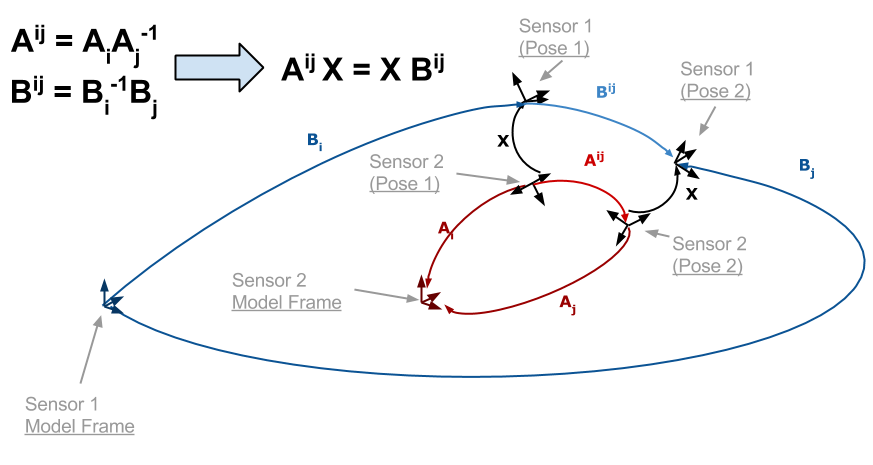
\includegraphics[width=3.3in]{figure/AX=XB(ASME)_v1.png}
\centering
\caption{The $AX=XB$  Sensor Calibration Formulation}
\label{AXXBfig1}
\end{figure}


\begin{figure}[t!]
\centering
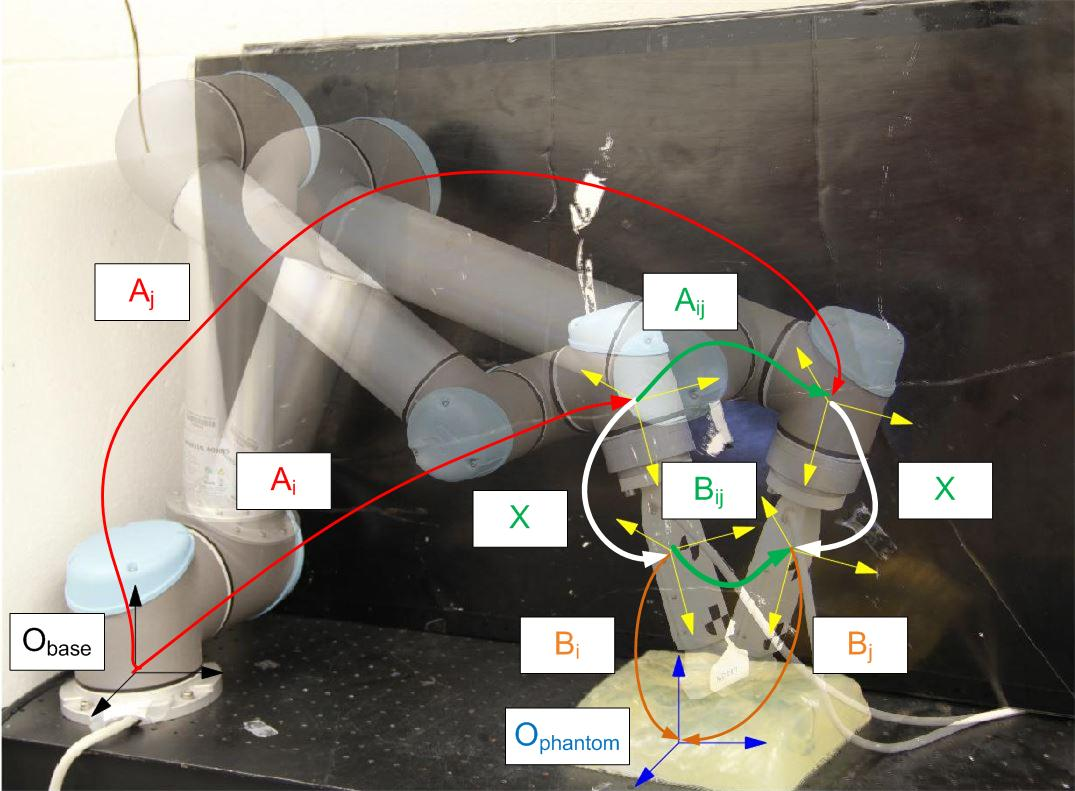
\includegraphics[width=3.3in]{Photos/UR5_Frame_Final.jpg}
\caption{Application of AX=XB in ultrasound sensor calibration: an ultrasound probe is attached to the end-effector and the calibration phantom is used for ultrasound probe calibration. (The UR5 robot pictured above is owned by Professor Emad Boctor of Johns Hopkins University)}
\label{AXXBfig2}
\end{figure}

\begin{figure}[t!]
\centering
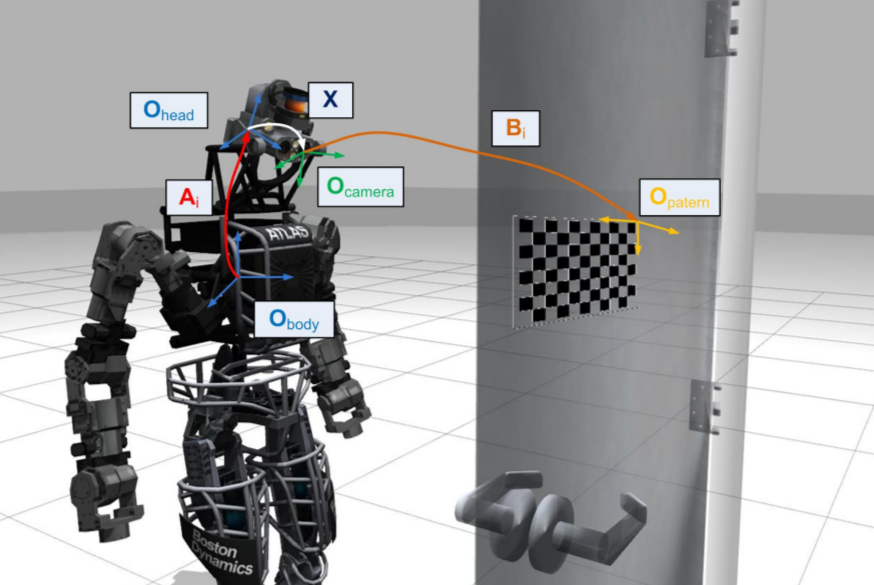
\includegraphics[width=3.3in]{Photos/Atlas_Humanoid.png}
\caption{Application of $AX=XB$ in Humanoid Camera Sensor Calibration: The Humanoid Robot Named Atlas Designed by
 \textit{Boston Dynamics} Requires head-body calibration before turning the knob. Different pairs of $(A_i, B_i)$ are measured by changing the head pose of the humanoid robot. (This picture was generated using the open-source robot simulation software Gazebo)}
\label{AXXBfig3}
\end{figure}


Performing the matrix multiplication of homogeneous transformations in Eq.~(\ref{mainaxxb}) and separating out the rotational and translational parts results in two equations of the form:
\begin{subequations}
\begin{gather}
R_A R_X = R_X R_B \label{subequ1}\\
R_A {\bf t}_X + {\bf t}_A = R_X {\bf t}_B + {\bf t}_X \label{subequ2}.
\end{gather}
\label{axxb}
\end{subequations}
One strategy for solving Eq.~(\ref{mainaxxb}) reduces to first solving Eq.~(\ref{subequ1}) for only rotation and then rearranging Eq.~(\ref{subequ2}) to find acceptable values of ${\bf t}_X$ satisfying $ (R_A - \mathbb{I}_{3}) {\bf t}_X = R_X {\bf t}_B - {\bf t}_A$.
%One strategy to solve Eq.~(\ref{mainaxxb}) \textcolor{blue}{of data}would appear to reduce to first solving Eq.~(\ref{subequ1}) for only rotation and then rearranging Eq.~(\ref{subequ2}) so as to find acceptable values of ${\bf t}_X$ satisfying $ (R_A - \mathbb{I}_{3}) {\bf t}_X = R_X {\bf t}_B - {\bf t}_A. $  
The other strategy is to solve for $R_{X}$ and $\ttt_{X}$ simultaneously based on some cost function $f(R_{X}, \ttt_{X})$ or reformulating the matrix equation into a dual quaternion representation. %dual quaternion. 
However, when there are only two exact sensor measurements, there are some problems with the first  approach. As pointed out in \cite{park1994robot,shiu1989calibration}, in nondegenerate cases, there is a one-parameter set of solutions to Eq.~\ref{subequ1}%the first part in Eq.(\ref{subequ1})
, and the matrix $R_A - \mathbb{I}_{3}$ in general has a rank of $2$. Hence, there are two unspecified degrees of freedom to the
problem, and it cannot be solved uniquely unless additional measurements are taken. 

Additionally, if there is sensor error, then it may not be possible to find compatible pairs that reproduce the exact value of $X$. For this reason, minimization approaches are often taken, where for $n>2$ a cost function:
\begin{equation}
C(X) = \sum_{i=1}^{n} w_i \, d^2(A_i X,X B_i)
\label{mainaxxb2}
\end{equation}
is computed for some distance metric $d(\cdot,\cdot)$ on $SE(3)$ and $\{w_i\}$ is a set of weights which can be taken as a partition of unity. 

This chapter is organized as follows. 
In Section~\ref{sec:sol_methods}, a detailed review is given for the existing methods that solve the $AX=XB$ problem using pairs of $\{A_{i}, B_{i}\}$ with correspondence. The notation used throughout the literature is not consistent and the authors strove %tried their best 
to standardize the notation used across the reviewed methods to provide the readers with a straightforward and consistent representation of the methods and their relationships.
Some approaches are preferable under certain circumstances and their advantages and disadvantages are also highlighted. 
In Section~\ref{sec:data_selection}, some important criterion for data selection and different errors metrics used in the literature are presented. 
Finally, in Section~\ref{sec:conclusion} a complete summary of the $AX=XB$ solvers is provided and open problems are noted as well.    

\section{EXISTING SOLUTION METHODS}
\label{sec:sol_methods}
 
The problem of solving Eq.~(\ref{mainaxxb}) for $X$ when multiple corresponding pairs of $A$s and $B$s are present has a history that stretches back more than a quarter of a century
\cite{chou1991finding, park1994robot,shiu1989calibration}, with the earliest proposed method introduced by Shiu \cite{shiu1987finding, shiu1989calibration} and Tsai \cite{tsai1989new}. Applications involving this problem still remain active today \cite{kim,dai}. Shah \cite{shah2012overview} overviewed several different AX = XB methods qualitatively. Fassi and Legnani \cite{fassi2005hand} gave a geometric view of $AX=XB$ and discussed the over-constrained and singular conditions. A more complete list of the traditional $AX=XB$ solvers includes: the Shiu method \cite{shiu1989calibration}, the screw motion method \cite{chen91,zhao2006hand}, the Euclidean group method \cite{park1994robot,gwak2003numerical}, the quaternion method\cite{chou1988quaternions, chou1991finding, horaud1995hand}, the dual quaternion method \cite{daniilidis1996dual, daniilidis1999hand}, and the Kronecker method \cite{andreff1999line,andreff2001robot}. Several new optimization methods emerged recently such as the convex optimization method \cite{zhao2011hand}, some global optimization methods  \cite{seo2009branch,andreff2001robot,heller2014hand} and a structure from motion (SfM) approach \cite{schmidt2005calibration}. The SfM method deals with the case where a calibration target is not applicable and a scaling factor needs to be calibrated in addition to rotation and translation. The methods mentioned previously are all off-line methods where $X$ can be calculated given a complete list of data pairs. However, several online methods have been 
proposed that are more preferable to real-time applications \cite{andreff1999line,angeles2000online,ackerman2014online}. All the methods above assume $\{A_i, B_i\}$ data pairs with correspondence. Probabilistic methods that deal with data pairs without correspondence are introduced in \cite{ackermanGSI, ackerman2014information}. In the follow sections, representatives of the above $AX=XB$ solvers will be reviewed in detail.

\begin{comment}
Decompose the 
\begin{equation}
AX = XB,
\label{AXXB}
\end{equation}
decompose Eq.(\ref{AXXB}) into the rotation component and the translation component: 
\begin{equation}
R_{A}R_{X} = R_{X}R_{B}
\label{Rotation}
\end{equation}
\begin{equation}
(R_{A} - I)\ttt_{x} = R_{X}\ttt_{B} - \ttt_{A}
\label{Translation}
\end{equation}
\end{comment}

\subsection{Shiu and Ahmad }
Shiu and Ahmad \cite{shiu1987finding,shiu1989calibration} use two data pairs $(A_{i}, B_{i})$ to solve for X. The necessary condition for the uniqueness of X is that the rotation axes of $R_{A_1}$ and $R_{A_2}$ are neither parallel nor anti-parallel, and the angles of rotation are neither 0 nor $\pi$. Though this method shows tolerance to noise to a certain extent, it is specifically designed to solve for the case where only two sets of $(A, B)$ are given. 
The rotation matrix $R_{X}$ is solved for first and the translation is obtained using a least squares technique given a known $R_{X}$.

The closed form expression for $R_{X}$ is:
\begin{equation}
R_{X} = \exp{(\hat{\nn}_{A}\beta)}R_{X_{P}}
\label{RotationCheng}
\end{equation}
where 
\begin{center}
$R_{X_{p}} =  \exp{(\widehat{\nn}_{X}\theta_{X})}$\\
$\nn_{X} = \nn_{B} \times \nn_{A}$\\
$\theta_{X} = \rm atan2(|\nn_{B} \times \nn_{A}|,\nn_{B} \cdot \nn_{A})$\\
\end{center}
and $\beta$ is an arbitrary angle. Given a vector $\nn = \left( n_{1}, n_{2}, n_{3} \right)^{T} \in \mathbb{R}^{3}$, $\widehat{\nn}$ is a skew-symmetric matrix defined as below:\\
\begin{equation}
\widehat{\nn}
=
\begin{pmatrix}
0 & -n_{3} & n_{2} \\
n_{3} & 0 & -n_{1} \\
-n_{2} & n_{1} & 0
\end{pmatrix}.
\end{equation}

Equation~(\ref{RotationCheng}) shows that $R_{x}$ has one degree of freedom which is determined by the angle $\beta$. Therefore, two relative arm motions are needed to generate two $(A_{i}, B_{i})$ data pairs in order to calculate the unique solution of $X$. Given two pairs of $A$s and $B$s, two equations can be obtained as:
\begin{subequations}
\begin{gather}
A_{1}X = XB_{1} \label{7a}\\
A_{2}X = XB_{2}.\label{7b}
\end{gather}
\end{subequations}
Instead of giving a closed-form solution, $R_{X}$ is calculated by solving for $\beta$ in Eq.~(\ref{CYD}), which is formulated as a system of linear equations obtained by equating two instances of Eq.~(\ref{RotationCheng}) that are obtained from data pairs $(A_{1}, B_{1})$ and $(A_{2}, B_{2})$:
\begin{equation}
CY = D.
\label{CYD}
%$${\color{red}(Detailed description of C and D?)}$$
\end{equation}
In Eq.~(\ref{CYD}), $Y = \big( \; \cos(\beta_{1}),\; \sin(\beta_{1}), \; \cos(\beta_{2}),\; 	\sin(\beta_{2}) \;\big)^{T}$ where $\beta_{1}, \, \beta_{2}$ correspond to Eq.~(\ref{7a}) and Eq.~(\ref{7b}) respectively,  $C \in \mathbb{R}^{9 \times 4}$ and $D \in \mathbb{R}^{9 \times 1}$ are determined from $\nn_{A_{1}}$, $\nn_{B_{1}}$, $\nn_{A_{2}}$, and $\nn_{B_{2}}$. The explicit expressions for $C$ and $D$ are given in Eq.~(44) of \cite{shiu1989calibration}.

Similarly, with known $R_{X}$, $\ttt_{x}$ can be calculated using the least squares method:
\begin{equation}
\bigg(\begin{array}{lr}
R_{A_{1}} - \mathbb{I}_{3} \\
R_{A_{2}} - \mathbb{I}_{3}
\end{array}\bigg)\ttt_{X}=
\bigg(\begin{array}{lr}
R_{X}\ttt_{B_{1}} - \ttt_{A_{1}}\\
R_{X}\ttt_{B_{2}} - \ttt_{A_{2}}
\end{array}
\bigg).
\label{trans}
\end{equation}
This is not a closed-form solution and it is constrained to the case where only two data pairs are provided. 

\subsection{Lie Group Method }
The Lie Group method \cite{park1994robot} by Park and Martin is the first method to solve the AX = XB problem from the perspective of Lie groups. It uses the axes of rotation of $A_{i}$ and $B_{i}$ to construct $R_{X}$ and gives both the closed-form solution for the no-noise case and the numerical solution for multiple noisy $(A_{i}, B_{i})$ pairs.
\subsubsection{Closed-Form Solution with Two Exact Pairs}
The closed-form solution for $R_{X}$ is as follows:
\begin{equation}
R_{X} = \mathcal{A}\mathcal{B}^{-1}
\label{Lie_Rotation}
\end{equation}
where\\

\begin{center}
$\mathcal{A} = (\nn_{A_{1}}, \nn_{A_{2}}, \nn_{A_{1}} \times \nn_{A_{2}}) \in \mathbb{R}^{3 \times 3}$\\
 $\mathcal{B} = (\nn_{B_{1}}, \nn_{B_{2}}, \nn_{B_{1}} \times \nn_{B_{2}}) \in \mathbb{R}^{3 \times 3} $\\
$\widehat{\nn}_{A_{1}} = \log(R_{A_{i}})/\|\log^\vee(R_{A_i})\|$\\
$\widehat{\nn}_{B_{1}} = \log(R_{B_{i}})/\|\log^\vee(R_{B_i})\|$
\end{center}
The solution for $R_X$ is uniquely determined given two pairs of $(A_i, B_i)$, and the solution for $\ttt_{X}$ can be obtained using Eq.~(\ref{trans}) once $R_{X}$ is obtained.\\
\begin{comment}
\begin{equation}
\bigg(\begin{array}{lr}
R_{A_{1}} - I \\
R_{A_{2}} - I
\end{array}\bigg)\ttt_{X}=
\bigg(\begin{array}{lr}
R_{X}\ttt_{B_{1}} - \ttt_{A_{1}}\\
R_{X}\ttt_{B_{2}} - \ttt_{A_{2}}
\end{array}
\bigg)
\label{Lie_Translation}
\end{equation}
\end{comment}

\subsubsection{Estimation of X Using Multiple Pairs with Noise}
When there are multiple pairs of $(A_{i}, B_{i})$ with noise, rotation matrix $R_{X}$ is solved for first and then the translation vector $\ttt_{x}$ is obtained using a least squares method given known $R_{X}$. The closed-form expression for $R_{X}$ is as follows:
\begin{equation}
R_{X} = (M^{T}M)^{-\frac{1}{2}}M^{T}
\end{equation}
where \\
\begin{center}
$M = \sum_{i=1}^{n}{\nn_{B_{i}} \nn_{A_{i}}^{T}}$.
\end{center}
Note that $i \geq 3$ is a necessary condition for $M$ to be a non-singular matrix, but it does not guarantee $M$ to be nonsingular. Theoretically, the Lie group method is more likely to fail when the number of data pairs is small, i.e., close to 3 pairs, while in real application, failure is rarely seen as long as the data pairs are not specially chosen such that M is degenerate. Given known $R_{X}$, $\ttt_{X}$ can be calculated using the least squares method shown in Eq.~(\ref{t_least}):

\begin{equation}
\ttt_{x} = (C^{T}C)^{-1}C^{T}d
\label{t_least}
\end{equation}
where\\

\begin{center}
$\begin{array}{lr}
C = \begin{pmatrix}
\mathbb{I}_{3} - R_{{A_{1}}}\\
\mathbb{I}_{3} - R_{{A_{2}}}\\
.\\
.\\
.\\
\mathbb{I}_{3} - R_{{A_{n}}}\\
\end{pmatrix}
\; \; 
& \; \;
d = \begin{pmatrix}
\ttt_{A_{1}} - R_{X}\ttt_{B_{1}}\\
\ttt_{A_{2}} - R_{X}\ttt_{B_{2}}\\.\\
.\\
.\\
\ttt_{A_{n}} - R_{X}\ttt_{B_{n}}\\\end{pmatrix} 
\end{array}$.
\end{center}


\subsection{Quaternion Method }
\label{sec:quats}
The Quaternion method proposed by Chou and Kamel \cite{chou1988quaternions,chou1991finding} uses unit quaternions to transform the rotation parts of $A_{i}X = XB_{i}$ (i = 1,2) into two linear systems. Then a singular value decomposition (SVD) is performed to obtain a closed-form solution for $R_{X}$. In order to estimate $X$ given multiple pairs of $(A_{i}, B_{i})$ with noise, Horaud and Dornaika \cite{horaud1995hand} cast the problem into a nonlinear optimization one. Two different approaches are discussed: (1) estimate the rotation matrix $R_{X}$ by minimizing an objective function, and solve for the translation $\ttt_{X}$ using a least squares method separately and (2) estimate $R_{X}$ and $\ttt_{X}$ simultaneously by minimizing an objective function that incorporates both the rotational and translational information. Method (1) turns out to have a closed-form solution for the unit quaternion $q_{X}$ representing the rotation $R_{X}$, while method (2) is a nonlinear optimization problem which requires an initial guess and will be discussed in Section~\ref{sec:optimization}. 
\subsubsection{Closed Form Solution with Two Exact Pairs}
\label{sec:quat_method}
First, the rotation equation in Eq.~(\ref{axxb}) is transformed into the equation of quaternion multiplication as below:
\begin{equation}
R_{A}R_{X} = R_{X}R_{B} 
\; \;
\Leftrightarrow
\; \;
q_{A}\odot q_{X} = q_{X}\odot q_{B}
\label{Quaternion}
\end{equation} 
where $q_{A}$, $q_{B}$ and $q_{X}$ are
unit quaternions that represent the rotation parts of matrices $A$, $B$ and $X$, and $\odot$ denotes quaternion multiplication.

Given two quaternions $q_{\alpha} = \left( \alpha_{0}, \alpha_{1}, \alpha_{2},\alpha_{3} \right)^{T} = \left( \alpha_{0}, \bf{\alpha}^{T} \right)^{T}$ and $q_{\beta} = \left( \beta_{0}, \beta_{1}, \beta_{2},\beta_{3} \right)^{T} = \left(\beta_{0}, \bf{\beta}^{T} \right)^{T}$, quaternion multiplication $\odot$ is defined as:
\begin{equation}
q_{\alpha}\odot q_{\beta} = 
\left(
\begin{matrix}
\alpha_{0} \beta_{0} - \bf{\alpha}^{T}\bf{\beta}\\
\alpha_{0}\bf{\beta} + \beta_{0}\bf{\alpha} + \bf{\tilde{\alpha}\beta}
\end{matrix}
\right).
\end{equation}
$\alpha_{0}$ is called the scalar component and $\bf{\alpha}$ is the vector component of the quaternion $q_{\alpha}$.
In order to solve for $q_{X}$, the quaternion equation is transformed into:
\begin{equation}
E\qq_{X} = \bf 0
\end{equation}
where $E \in \mathbb{R}^{4 \times 4}$ is obtained by grouping $q_{A}$ and $q_{B}$ together, and $\qq_{X} \in \mathbb{R}^4$ is the vector representation of the unit quaternion ${q_X}$.\\

It turns out that the unit quaternion $q_X$ which represents the rotation part of $X$ can be written as: 
\begin{equation}
\qq_{X} = V_{2}\bf y_{2}.
\label{QuaternionUnit}
\end{equation}
To obtain the matrix $V_{2}$ and vector $y_{2}$, $E$ is first written as $E =  \sin(\theta_{A|B}/2)E_0$ with $\theta_{A|B} = \theta_{A} = \theta_{B}$, which is the constraint that the corresponding transformations $A_i$ and $B_i$ should have the same angle of rotation. Next, the SVD of $M$ is computed as $E_0 = U\Sigma V^{T}$ where $V = (V_{1}, V_{2})$,  $V_{1} \in \mathbb{R}^{4 \times 2}$, $V_{2} \in \mathbb{R}^{4 \times 2}$, $U \in \mathbb{R}^{4 \times 4}$ and $\Sigma$ is a diagonal matrix. Vector ${\bf y_{2}}$ is obtained by calculating ${\bf y} =  V^{T}\qq_{x}$ where $\bf y = (\bf y^{T}_{1},\bf y^{T}_{2} )^{T}$, ${\bf y_{1}} \in \mathbb{R}^{2 \times 1}$ and ${\bf y_{2}} \in \mathbb{R}^{2 \times 1}$. Their expressions are also outlined as follows:\\

\begin{center}
$\begin{array}{lcl}
E & = & \sin(\theta_{A|B}/2)E_0\\
M & = & U\Sigma V^{T}\\
V & = & (V_{1}, V_{2})\\
\bf y & = & V^{T}\qq_{x}\\
\bf y & = & (\bf y^{T}_{1},\bf y^{T}_{2} )^{T}.
\end{array}$
\end{center}
The translation vector $\ttt_{x}$ satisfies the following equation:
%{\color{red} write equation of $\ttt_{x}$ in a more concise form by substituting c = (A-I)}
%\begin{equation}
%\ttt_{x} = {\bf \nn_{A}} z - \frac{1}{2}\bigg( \cot(\frac{\theta_{A}}{2})\hat{\nn}_{A} + I %\bigg){\bf c}
%\end{equation}
\begin{equation}
\left(\cot(\dfrac{\theta_{A}}{2})\hat{\nn}_{A}(R_{A}-\mathbb{I}_{3})+ R_{A} + \mathbb{I}_{3}\right)\ttt_{x} = \nn_{A}z
\label{QuaternionTranslation} 
\end{equation}
%\begin{equation}
%{\bf c = (R_{A} - I)\ttt_{x}} \;\; \text{  and  } \;\; z \in \mathbb{R} \text{  is arbitrary} 
%\label{QuaternionTranslation}
%\end{equation}
where $z \in \mathbb{R}$ is arbitrary. A unique solution can be calculated using Eq.~(\ref{QuaternionUnit}) and Eq.~(\ref{QuaternionTranslation}) given two nondegenerate pairs of $(A_{i}, B_{i})$.

\subsubsection{Estimation of X Using Multiple Pairs With Noise}
As shown in \cite{horaud1995hand}, in the case where there are n pairs of $(A_{i}, B_{i})$, the problem of recovering $R_{X}$ is converted into minimizing the following error objective function:
\begin{equation}
\begin{array}{c}
f(R_{X})
= \sum_{i = 1}^{n}||{n_{A_{i}} - q_{X} \odot n_{B{i}} \odot \bar{q}_{X}}||^{2} \\
\\ 
= {\qq_{X}}^{T}\tilde{K}{\qq_{X}}
\end{array}
\label{ErrorQuaternion} 
\end{equation}
where $n_{A_{i}} = \left(0, {\nn_{A_{i}}}^{T}\right)^{T}$ and $n_{B_{i}} = \left(0, {\nn_{B_{i}}}^{T}\right)^{T}$. $\tilde{K} = \sum_{i = 1}^{n}\tilde{K_{i}}$ and $\tilde{K_{i}} \in \mathbb{R}^{4 \times 4}$ is a symmetric positive definite matrix determined by $\nn_{A_{i}}$ and $\nn_{B_{i}}$; $\bar{q}_{X}$ is the conjugate of ${q}_{X}$ where $q_{X} \odot \bar{q}_{X} = 1$.

To minimize  Eq.~(\ref{ErrorQuaternion}) under the constraint that $\qq_{X}$ is a unit quaternion, the Lagrangian multiplier is introduced as:
\begin{equation}
\min_{q} f = \min_{q}({\qq_{X}}^{T}\tilde{K}{\qq_{X}} + \lambda(1 - {\qq_{X}}^{T}{\qq_{X}})).
\label{ErrorLagrangeMultiplier}
\end{equation}
Differentiating the error function with respect to $\qq_{X}$, the 1st order necessary optimality condition is obtained as: 
\begin{equation}
\tilde{K}\qq_{X} = \lambda \qq_{X}.
\label{QuaternionEig}
\end{equation}
It can be shown that the unit quaternion $\qq_{X}$ that minimizes $f$ is the eigenvector of $\tilde{K}$ associated with its smallest positive eigenvalue. After recovering $\qq_{X}$ (or equivalently $R_{X}$), $\ttt_{X}$ can be recovered using the least square techniques introduced in previous methods.

\subsection{Dual Quaternion Method }
The dual quaternion method proposed by Daniilidis and Bayro-Corrochano \cite{daniilidis1996dual} (Daniilidis \cite{daniilidis1999hand}) treats the rotation and translation parts of the matrix X in a unified way and facilitates a new simultaneous solution of X using SVD. To begin, Eq.~(\ref{mainaxxb}) is transformed into an equation of dual quaternions: %in dual quaternion form as follows:
\begin{equation}
AX = XB 
\; \;
\Leftrightarrow
\; \;
\check{a} = \check{q}_{X}\hat{\odot}\check{b}\hat{\odot}\bar{\check{q}}_{X}
\label{DualQuaternion}
\end{equation}
where $\check{a}$, $\check{b}$ and $\check{q}$ are the dual quaternions that represent matrices $A$, $B$ and $X$, and $\bar{\check{q}}$ is the conjugate of $\check{q}$.

The dual quaternion that corresponds to a 4x4 %4 by 4 
rigid transformation matrix is defined as follows:
\begin{equation}
\check{q}_{X} =
\Bigg( 
\begin{array}{c}
\cos(\frac{\theta + \epsilon d}{2})\\
\sin(\frac{\theta + \epsilon d}{2})({\bf l} + \epsilon {\bf m})
\end{array}
\Bigg)
\label{dual_screw}
\end{equation}
where
$\theta$, $d$, ${\bf l}$ and ${\bf m}$ are screw parameters and ${\epsilon}^{2} = 0$. $\theta$ is the rotation angle, $d$ is the pitch, $\vec{\bf l}$ is the direction of the screw, and ${\bf m} = {\bf p} \times {\bf l}$ is the line moment where ${\bf p}$ is a point on the line. The six tuple $({\bf l}, {\bf m})$ defines a line in 3-D space. Furthermore, by expanding the dual terms in $\check{q}_{X}$, Eq.~(\ref{dual_screw}) can also be written as:
\begin{equation}
\check{q}_{X} = q_{X} + \epsilon {q}^{\prime}_{X}.
\end{equation} 
Both $q$ and $q^{\prime}$ are quaternions satisfying the following constraints:
\begin{equation}
{\bf q}^{T}_{X}{\bf q}_{X} = 1 \; \; \text{and} \;
\; {\bf q}^{T}_{X}{\bf q}^{\prime}_{X} = 0
\end{equation}
where ${\bf q}_{X}$ and ${\bf q}^{\prime}_{X}$ are the vector representations of $q_{X}$ and $q^{\prime}_{X}$.
Then equation $A_{i}X = XB_{i}$ can be converted into the form below:

\begin{equation}
S_{i}
\underbrace{
\bigg(
\begin{array}{c}
{\bf q}_{X}\\
{\bf q}^{\prime}_{X}
\end{array}
\bigg)}_{\xx} = \bf 0
\label{dqua}
\end{equation} 
where
\begin{equation}
S_{i} = 
\bigg(
\begin{array}{cccc}

{\aaa} - {\bbb} & \; ({\aaa} + {\bbb})^{\wedge} & \; \bf 0_{3\times 1} & \bf 0_{3\times 3}\\

{\aaa}^{\prime} - {\bbb}^{\prime} & ({{\aaa}^{\prime} + {\bbb}^{\prime}})^{\wedge} & {\aaa} - {\bbb} & ({\aaa} + {\bbb})^{\wedge} 

\end{array}
\bigg) \in \mathbb{R}^{6 \times 8}.
\end{equation}
The notation for $\bf x$ here will be also used in Section %3.6. 
To maintain the consistency of notation throughout the chapter as well as preserve the original notation in \cite{daniilidis1996dual}, for a vector ${\bf v} \in \mathbb{R}^{3 \times 1}$, ${\bf v}^{\wedge}$ is the same as $\tilde{\bf v}$ which maps a vector into the corresponding skew-symmetric matrix. ${\aaa}^{\prime} = \dfrac{1}{2}{\ttt}_{X} \times {\aaa}$ and $\aaa$ is the vector part of $q_{X}$. Similarly,  $\bbb$ is the vector part of $q^{\prime}$.
After concatenating $S_{i}$, the following matrix $T$ can be obtained and used to solve for $X$:
\begin{equation}
T = \big( \; \; S_{1}^{T} \; S_{2}^{T} \; \; ... \; \; S_{n}^{T} \; \; \big)^{T}.
\end{equation}
By calculating the SVD of $T = U\Sigma V^{T}$, the dual quaternion for matrix X can be expressed as a linear combination of the last two right-singular vectors (${\bf v_{7}}$, ${\bf v_{8}}$) of matrix $T$, which are the last two columns of matrix $V$, as shown below: 
\begin{equation}
\bigg(
\begin{array}{c}
{\bf q}_{X}\\
{\bf q}^{\prime}_{X}
\end{array}
\bigg) = 
\lambda_{1}{\bf v_{7}} + \lambda_{2}{\bf v_{8}} \in \mathbb{R}^{8} \; \;
\text{where} \; \; \lambda_{1}, \lambda_{2} \in \mathbb{R}.
\label{dq_closed}
\end{equation} 

Different from the quaternion method in \ref{sec:quat_method}, the dual quaternion method solves the rotational part and translational part in a united way, and it contains all the information to reconstruct matrix $X$. However, it does not use all of the available information, only the imaginary parts of $\check{a}$ and $\check{b}$. Despite the advantages of the dual quaternion method, its major drawback is the need to filter the data pairs to ensure appropriate solutions when there is noise on $A_{i}$ and $B_{i}$.

\subsection{Kronecker Product Method }
\label{sec:Kronecker}
Inspired by the well known Sylvester equation ( $AX + XB = C$ ) in linear systems, Andreff {\it et al}. \cite{andreff1999line} proposed the Kronecker method which converts  Eq.~(\ref{mainaxxb}) into the form of Kronecker products \cite{andreff1999line}: % as in Eq.~(\ref{KroneckerMethod}):
\begin{equation}
\begin{split}
AX &= XB  \Leftrightarrow\\
\underbrace{\Bigg(
\begin{array}{cc}
\mathbb{I}_{9} - R_{B} \otimes R_{A} \; & \; 0_{9 \times 3}\\
\ttt_{B}^{T} \otimes \mathbb{I}_{3} & \mathbb{I}_{3} - R_{A}
\end{array}
\Bigg)}_{C}
&\underbrace{\Bigg(
\begin{array}{c}
vec(R_{X})\\
\ttt_{X}
\end{array}
\Bigg)}_{\bf x} =
\underbrace{
\Bigg(
\begin{array}{c}
0_{9}\\
\ttt_{A}
\end{array}
\Bigg)}_{d}.
\end{split}
\label{KroneckerMethod}
\end{equation}
where $C, d, \bf x$ will be referred to in Section~\ref{sec:optimization}. 
%where the symbol $\otimes$ denotes the Kronecker product. The $vec$ operator was introduced in \cite{neudecker1969note} and it's used to reorder the $m \times n$ components of a matrix $M_{m \times n}$ into a $mn$ vector $vec(M_{m \times n})$.\\
Given multiple pairs of $A$s and $B$s with noise, the Kronecker product is reformulated as:% Eq.(\ref{KroneckerRotation}) and Eq.(\ref{KroneckerTrans}):
\begin{equation}
\left(
\begin{array}{c}
\mathbb{I}_{9} - R_{B_{1}} \otimes R_{A_{1}}\\
\mathbb{I}_{9} - R_{B_{2}} \otimes R_{A_{2}}\\
\vdots\\
I_{9} - R_{B_{n}} \otimes R_{A_{n}}
\end{array}
\right) 
vec(R_{X})
 = {\bf{0}}_{9 n \times 1},
\label{KroneckerRotation}
\end{equation}
and
\begin{equation}
\left(
\begin{array}{c}
\mathbb{I}_{3} - R_{A_{1}} \\
\mathbb{I}_{3} - R_{A_{2}} \\
\vdots\\
\mathbb{I}_{3} - R_{A_{n}}
\end{array}
\right) 
{\ttt_{X}}
 = 
\left( 
\begin{array}{c}
{\bf{t}}_{A_{1}} - R_{X}{\bf{t}}_{B_{1}}\\
{\bf{t}}_{A_{2}} - R_{X}{\bf{t}}_{B_{2}}\\
\vdots\\
{\bf{t}}_{A_{n}} - R_{X}{\bf{t}}_{B_{n}}\\
\end{array}
\right).
\label{KroneckerTrans}
\end{equation}
The vectorized version of $R_X$ obtained from Eq.~(\ref{KroneckerRotation}) is not an element of $SO(3)$ and
orthogonalization on $R_{X}$ is required to obtain a rotation matrix:% as in Eq.~(\ref{Orthogonolization}):
\begin{equation}
R_{X_{e}} = R_{X}(R_{X}^{T}R_{X})^{-1/2}
\label{Orthogonolization}
\end{equation}
\cite{horn1986robot}
where $R_{X_{e}}$ denotes the orthogonalized $R_{X}$.

The orthogonalized matrix $R_{X_{e}}$ is further normalized as: % in Eq.(\ref{kron_normal}): 
\begin{equation}
R_{X_{n}} = \dfrac{sign(\textrm{det}(R_{X_{e}}))}{{|\textrm{det}(R_{X_{e}})|}^{\tfrac{1}{3}}}R_{X_{e}}
\label{kron_normal}
\end{equation}
where $R_{X_{n}}$ is the normalized matrix of $R_{X_{e}}$.
After getting the estimation of $R_{X}$, a least squares method is implemented on Eq.~(\ref{KroneckerTrans}) to recover $\ttt_{X}$. One advantage of the Kronecker product method is its capability of dealing with small motions, because the associated orthogonal matrix $R_{X_{n}}$ is always defined, while the rotation can be ill-defined when using the axis-angle representation. Moreover, the linear system can also be used to analyze.

 the  recoverable information in $X$ based on the available type and number of motions. Details are included in Section \ref{sec:data_selection}. In addition, an on-line hand-eye calibration method is developed for an unknown scene based on the above algorithm, where the camera translations are estimated up to a scaling factor. 

\subsection{Optimization Methods}
\label{sec:optimization}
Different optimization methods have been proposed in the literature and most of them are built upon the various parametrizations of the $AX=XB$ equations mentioned previously. 
\subsubsection{Quaternion Based Simultaneous Approach}
When trying to solve for $R_{X}$ and $\ttt_{X}$ simultaneously, it is impossible to find a closed-form solution. Horaud and Dornaika \cite{horaud1995hand} presented an objective function for minimization, which is a sum of squares of nonlinear functions as:
\begin{equation}
\begin{split}
f(q_X,\ttt_{X}) = \lambda_{1} \sum_{i = 1}^{n}||vec(q_{X} \odot t_{B_{i}} \odot \bar{q}_{X}) -(R_{A_i} - \mathbb{I})\ttt_{X} - \ttt_{A_i}||^{2}\\
+ \lambda_{2} \sum_{i = 1}^{n}||{n_{A_{i}} - q_{X} \odot n_{B_{i}} \odot \bar{q}_{X}}||^{2} + \lambda_{3}(1 - \qq_{X}^{T}\qq_{X})^2
\end{split}
\label{simlqua}
\end{equation}
where $\lambda_1, \lambda_2, \lambda_3 \in \mathbb{R}$. Note that $vec()$ here represents the vector part of a quaternion such that $vec(q) \in \mathbb{R}^{3}$. The third term is a penalty function where the modulus %module 
of $q$ will approach 1 when $\lambda_{3}$ becomes large. This is a non-convex optimization problem which requires a good initial guess due to the existence of multiple local minima. However, the result can be more accurate than the rest of the solvers for certain motion pairs when the initial guess is ``good".

\subsubsection{Polynomial Global Optimization}
Heller {\it et al.} \cite{heller2014hand} developed a polynomial global optimization method which does not require an initial estimate and is also globally optimal in the $L_2$-norm sense. Defining a certain parametrization of $X \in SE(3)$ as $P(X)$, the previous minimization problem Eq.~(\ref{mainaxxb2}) is formulated as:
\begin{equation}
\begin{split}
&\underset{X \in SE(3)}{\text{min}}\sum_{i=1}^n ||A_{i}X - XB_{i}||^2 \Leftrightarrow \\
&\text{minimize} \; \; \; \; f(P(X)) \\
\; \; &\text{subject to} \; \; {\bf c}(P(X)) \geq {\bf 0} 
\end{split}
\label{LMI}
\end{equation}
where $f(X)$ is the converted multivariate polynomial function using the convex linear matrix inequality (LMI) relaxations technique \cite{lepetit2009epnp}. 

When $R_X$ is parametrized using the orthonormal basis as $R_{X}(\uu, \vv) = ( \uu, \vv, \uu \times \vv)$ where $\vv, \uu \in \mathbb{R}^{3}$, then Eq.~(\ref{LMI}) becomes:
\begin{equation}
\begin{split}
\text{minimize} \; \; \; \;&f_{1}(\uu, \vv, \ttt_{X}) = \\
&\sum_{i=1}^n ||A_i X(\uu,\vv,\ttt_{X}) - X(\uu,\vv,\ttt_{X})B_i ||^2\\
\text{subject to} \; \; \; \; &\uu^{T}\uu = 1, \vv^{T}\vv = 1, \uu^{T}\vv = 0.
\end{split}
\label{orLMI}
\end{equation}
Similarly, using the quaternion representation of $R_{X}$, Eq.~(\ref{LMI}) becomes:
\begin{equation}
\begin{split}
\text{minimize} \; \; \; \; &f_{2}(\qq_{X}, \ttt_{X}) = \\
& \sum_{i=1}^{n}||A_iX(\qq_{X}, \ttt_{X}) - X(\qq_{X}, \ttt_{X})B_i||^{2}\\
\text{subject to} \; \; \; \; &\qq_{X}^{T}\qq_{X} = 1, \; \; q_{X1} \geq 0.
\end{split}
\label{qLMI}
\end{equation}
If $A$, $B$ and $X$ are parametrized using dual the quaternion representation, then
\begin{equation}
\begin{split}
\text{minimize} \; \; \; \; &f_{3}(\check{q}_{X}) = \\
 & \sum_{i=1}^{n}||\check{q}_{A} \hat{\odot} \check{q}_{X}- \check{q}_{X} \hat{\odot} \check{q}_{B}||^{2}\\
\text{subject to} \; \; \; \; &\qq_{X}^{T}\qq_{X} = 1, \; \; q_{X1} \geq 0 \\
&q_{X1}q_{X5} + q_{X2}q_{X6} + q_{X3}q_{X7} + q_{X4}q_{X8} = 0.
\end{split}
\label{dqLMI}
\end{equation} 
As pointed out in \cite{heller2014hand}, the polynomial global optimization method as described in Eq.~(\ref{dqLMI}) can give better solutions than Park \cite{park1994robot}, Eq.~(\ref{simlqua}), Eq.~(\ref{orLMI}) and Eq.~(\ref{qLMI}). For those who are also interested in robot-world and hand-eye calibration, several solvers for $AX=YB$ 
using the LMI technique are also given; however, they fail to give better results than the traditional methods.
\subsubsection{Convex Optimization}
Based on different ways of formulating the rotation part of the rigid body transformation, Zhao \cite{zhao2011hand} gives two formulations that use a $L_\infty$ optimization technique. $L_\infty$ optimization is the minimax problem:
\begin{equation}
\underset{\bf x}{\text{min}} \; \; \underset{i}{\text{max}} f_{i}(\bf x) \; \; i = 1,2,... ,n
\label{convex}
\end{equation} 
where $\bf x$ represents all the unknown transformation parameters and $f_{i}(\xx)$ is the error function corresponding to $(A_i, B_i)$. Eq.~(\ref{convex}) can be converted into a convex optimization problem if $f_i(\bf x)$ is a quasi-convex function on a convex domain on which it is to be minimized.  

Using the Kronecker formulation as in Eq.~(\ref{KroneckerMethod}) and introducing an additional variable $\delta$, the equivalent form of the $L_\infty$ optimization problem is:
\begin{equation}
\begin{split}
&\underset{\delta, \xx}{\text{min}} \; \; \delta \\
&\text{subject to} \; \; ||C_i\xx - {\bf d}_i||_2 \leq \delta \\
&\text{where} \; \; i = 1,2,...,n.
\end{split}
\end{equation}
The matrix ${\bf C}_i$, vector $\bf x$, and ${\bf d}_i$ correspond to those in Eq.~(\ref{KroneckerMethod}).
Above is a convex optimization problem that can be solved using a \textit{second-order cone program}, which can be solved using toolboxes available online. 

When the $AX=XB$ problem is formulated as a dual quaternion representation as in Eq.~(\ref{dqua}), the equivalent $L_\infty$ optimization problem can be written as:
\begin{equation}
\begin{split}
&\underset{\delta, \xx}{\text{min}} \; \; \delta \\
&\text{subject to} \; \; ||S_i\xx||_2 \leq \delta \\
&\text{where} \; \; i = 1,2,...,n \; \; \text{with} \; \; \bf{Dx \geq f}.
\end{split}
\end{equation}
The matrix $S_i$ and vector $\bf x$ correspond to those in Eq.~(\ref{dqua}). 
The inequality constraint $\bf{Dx \geq f}$ is added manually in order to prevent $\xx$ from reaching zero, which is a meaningless solution for the program. $\bf x$ must also satisfy two additional constraints: $\|\qq_X\|=1$ and $\|\qq_{X}^{\prime}\|=1$. %Another constraint $\bf x$ has to satisfy is that $||\qq_X||=1$ and $||\qq_{X}^{\prime}||=1$.

The proposed methods need no initial guess and are less time consuming compared to the simultaneous optimization method given in Eq.~($\ref{simlqua}$). However, the errors for both of the convex optimization methods are larger than the latter. 
\subsection{Gradient Descent Method}
Except for the Kronecker product method, all the methods mentioned above are only able to solve for matrix $X$ offline, which means $\{A_{i}, B_{i}\}$ data pairs should be fully collected before being put into the algorithm. The gradient descent method \cite{ackerman2014online} by Ackerman {\it et al.} is an online sensor calibration method which uses a gradient descent optimization on the Euclidean group (SE(3)) given an appropriate cost function. 

To begin, define $\mathcal{X} \in se(3)$ as the Lie algebra corresponding to $G = SE(3)$, and let $f:G \rightarrow \mathbb{R}$ be an analytic function and $g \in G$. As defined in \cite{myoldbook}, the concept of directional derivatives in $\mathbb{R}^{n}$ is extended to functions on a Lie group as:
\begin{equation}
\left.(\hat{\mathcal{X}}^{r}f)(g)\doteq \dfrac{d}{dt}f(g\circ \text{exp}(t\mathcal{X}))\right\vert_{t=0}.
\label{r_lie_d}
\end{equation}
Note that $t$ is just a scalar denoting the time, while $\ttt$ represents the translation part of a homogeneous transformation.
Eq.~(\ref{r_lie_d}) is the ``right'' Lie derivative and the ``left'' Lie derivative can be defined in a similar form. A gradient on $SE(3)$ is then defined using the right Lie derivative with the ``natural'' basis of Lie algebra $\{E_{i}\}$ where $i = 1,2,...,6$. Therefore, the gradient of the function on Lie group $f(g)$ is as follows:
\begin{equation}
\nabla f(g)= \left( 
\begin{matrix}
\frac{d}{dt}\left.f(g\circ \text{exp}(tE_{1}))\right\vert _{t=0} \\
\frac{d}{dt}\left.f(g\circ \text{exp}(tE_{2}))\right\vert _{t=0} \\
\vdots \\
\frac{d}{dt}\left.f(g\circ \text{exp}(tE_{6}))\right\vert _{t=0}
\end{matrix}
\right).
\end{equation}

In order to update $g$, the rigid body velocity is introduced where $V^{r}_{g} = g^{-1}\dot{g}$, and the update law is written as below:
\begin{equation}
g_{s+1} = g_{s}\text{exp}(\Delta t V^{r}_{g})
\end{equation}
where $t_{s+1} = t_{s} + \Delta t$ is the discrete time step corresponding to $g_{s+1}$. To prevent steps from becoming too small, the update law of $g_s$ is modified by defining $V^{r}_{g}$ as:
 
\begin{equation}
V^{r}_{g} = g^{-1}\dot{g} = -\alpha \widehat{\nabla f(g)}.
\label{gs}
\end{equation} 
where $\alpha$ is a scaling factor.
After choosing the cost function as:
\begin{equation}
C(X) = \sum_{i=1}^{n}||A_{i}X - XB_{i}||
\end{equation}
$X$ can be optimized using Eq.~(\ref{gs}).
The gradient descent method updates the calibrations parameters online based on new incoming data. The initial guess of $X$ will converge to the true $X$; however, the rate of convergence depends on how ``good'' the initial guesses are.


\subsection{Batch Method}
\label{batchnoisefree}
This section presents a probabilistic method \cite{ackermanGSI} by Ackerman and Chirikjian to solve for $X$ in the absence of %when there does not need to be any 
a priori knowledge of the correspondence between the exact sets of measurements
$A = \{A_i\}$ and $B = \{B_j\}$. In other words, the sets $A$ and $B$ each can be given as unordered ``batches'' without knowing how each $A_i$ matches to a specific $B_j$.

A commonality of all the methods in the previous sections is that exact knowledge of the correspondence between $\{A_i\}$ and $\{B_j\}$ is assumed; however, this is not always the case. There are many instances in the literature when the sensor data used in calibration becomes ``unsynchronized''. Different attempts have been implemented to solve this problem, such as time stamping the data, developing dedicated software modules for syncing the data, and analyzing components of the sensor data stream to determine a correlation \cite{darius1}, to varying effects. The Batch method bypasses these issues altogether without tracking, or recomputing, correspondence. By modelling the set of $A$s and $B$s as probability distributions on $SE(3)$, the data can be taken as an unordered, uncorrelated ``batch" and a solution for $X$ can be generated.

\subsubsection{The Batch Method Formulation}
Given a large set of pairs $(A_i,B_i) \in SE(3) \times SE(3)$ for $i =1,...,n$ that exactly satisfy the equation:
\begin{equation} A_i X = X B_i , \label{main} \end{equation}
a new algorithm is developed to find $X \in SE(3)$. The Batch method addresses a generalization of the standard problem in which
the sets $A=\{A_i\}$ and $B =\{B_j\}$ are provided with elements written in any order and it is known that a correspondence exists between the elements of these sets such that Eq.~(\ref{main}) holds, but no a priori knowledge of this correspondence is known between each $A_i$ and $B_j$.

Define a Gaussian probability distribution on $SE(3)$ (assuming the norm $\|\Sigma\|$ is small) as:
$$ \rho(H; M, \Sigma) = \frac{1}{(2\pi)^3 |\Sigma|^{\half}} e^{-\half F(M^{-1} H)} $$
where $|\Sigma|$ denotes the determinant of $\Sigma$ and
$$ F(H) = [\log^{\vee}(H)]^T \Sigma^{-1} [\log^{\vee}(H)]. $$
When $H$ is parameterized with exponential coordinates, $H = \exp Z$, this means that
$F(\exp Z) = {\bf z}^T \Sigma^{-1}  {\bf z}$ where ${\bf z} = Z^{\vee}$ and
$\rho(\exp Z; \mathbb{I}_4, \Sigma)$ becomes exactly a zero-mean Gaussian distribution on the Lie algebra $se(3)$, with covariance $\Sigma$, that is `lifted up' to the Lie group $SE(3)$. This definition is valid when $\|\Sigma\|$ is small enough that the tails of the distribution decay rapidly enough such that the value of $\rho$
becomes negligible before they ``wrap around'' due to the topology of $SE(3)$. 

Using formulations of probability theory on SE(3), Eq.~(\ref{main}) can be thought as:
\begin{equation} (\delta_{A_i} * \delta_X)(H) = (\delta_X * \delta_{B_i})(H) \label{mainconv} \end{equation}
where $*$ denotes the convolution of functions on $SE(3)$, as defined in the Appendix.
\begin{comment}
Whereas the addition (as opposed to multiplication) of homogeneous transformation matrices is nonsensical, the addition of real-valued functions $f_1(H) + f_2(H)$ is a perfectly reasonable operation and
\end{comment}

Because convolution is a linear operation on functions, the following equation can be obtained by adding all $n$ instances of Eq.~(\ref{mainconv}):
\begin{equation} (f_A * \delta_X)(H) = (\delta_X * f_B)(H) \label{mainconvall} \end{equation}
where $$ f_A(H) = \frac{1}{n} \sum_{i=1}^{n} \delta(A_i^{-1} H) \,\,\, {\rm and} \,\,\, f_B(H) = \frac{1}{n} \sum_{i=1}^{n} \delta(B_i^{-1} H). $$
The above functions can be normalized
to be probability densities:
$$ \int_{SE(3)} f_A(H) dH = \int_{SE(3)} f_B(H) dH = 1. $$
See the Appendix for a review of the properties of integration on $SE(3)$.

Let the mean and covariance of a probability density function $f(H)$ be defined by the following conditions:
\begin{equation} \begin{split} &\int_{SE(3)} \log(M^{-1} H) f(H) dH = \mathbb{O} \,\,\, {\rm and} \,\,\,\\ &\Sigma = \int_{SE(3)} \log^{\vee}(M^{-1} H) [\log^{\vee}(M^{-1} H)]^T  f(H) dH . \end{split}\label{meancovdef} \end{equation}
If $f(H)$ is of the form of $f_A(H)$ given above, then
\begin{equation} \
\begin{split} &\sum_{i=1}^{n} \log(M_A^{-1} A_i) = \mathbb{O} {\rm \,\,\,\,\, and} \\
&\Sigma_A = \frac{1}{n} \sum_{i=1}^{n} \log^{\vee}(M_A^{-1} A_i) [\log^{\vee}(M_A^{-1} A_i)]^T.  \label{datameancovconvdef} \end{split}
\end{equation}

It can be shown that if these quantities are computed for two highly-focused functions, $f_1$ and $f_2$, that the same quantities for
the convolution of these functions can be closely approximated as \cite{Wang08}:
\begin{equation}
M_{1*2} = M_1 \, M_2 \,\,\, {\rm and} \,\,\, \Sigma_{1*2} = Ad(M_2^{-1}) \,\Sigma_{1}\, Ad^T(M_2^{-1}) + \Sigma_{2}
\label{meancovconvdef} \end{equation}
where
\begin{equation} 
Ad(H) = \left(\begin{array}{ccc}
R && \mathbb{O} \\
\widehat{{\bf x}} R && R \end{array}\right) 
\label{adjdef} \end{equation}
and $\widehat{{\bf a}}$ is the skew-symmetric matrix such that $\widehat{{\bf a}} {\bf b} = {\bf a} \times {\bf b}$.

The mean of $\delta_X(H)$ is $M_X = X$, and its covariance is the zero matrix.
Therefore, Eq.~(\ref{mainconvall}) together with Eq.~(\ref{meancovconvdef}) yields two ``Batch Method" equations:
\begin{equation}
\boxed{\,
M_A \, X = X \, M_B
\,}
\label{mainmain11} \end{equation}
and
\begin{equation}
\boxed{\,
Ad(X^{-1}) \, \Sigma_{A} \, Ad^T(X^{-1}) = \Sigma_{B}
\,}
\label{mainmain12} \end{equation}
In Section~\ref{sec:batch_meth_sol}, it will be shown how $X$ can be recovered using Eq.~(\ref{mainmain11}) and Eq.~(\ref{mainmain12}).

\subsubsection{A Batch Method Solution}
\label{sec:batch_meth_sol}
Starting with Eq.~(\ref{mainmain11}), the solution space of $X$ can be defined as a cylinder. Specifically Eq.~(\ref{mainmain11}) can be rewritten as:

\begin{equation}
\log^{\vee}(M_A)  = Ad(X) \,\log^{\vee}(M_B).
\label{mainmain1rewrite} \end{equation}

In the case of general $M_A$ and $M_B$ (i.e. not degenerate cases in which the rotation angle\footnote{This angle is computed from the Frobenius norm $\theta_A =\|\half \log R_A\| = \|\half \log R_B\|= \theta_B$.} is outside of the range
$(0,\pi)$), the solution space of all possible $X$s that satisfy this equation is known to be two-dimensional.
This can be seen by defining
$$ \log^{\vee}(M) = \left(\begin{array}{c}
\omega \\
{\bf v} \end{array} \right)
=\left(\begin{array}{c}
\theta \, {\bf n} \\
{\bf v} \end{array} \right), $$
where ${\bf \omega} \in \mathbb{R}^3$ and ${\bf v} \in \mathbb{R}^3$ are the elements of the Lie algebra, and writing the rotation and translation parts of Eq.~(\ref{mainmain1rewrite}) separately,
\begin{equation}
{\bf n}_A = R_X {\bf n}_B \hspace{5mm}\mbox{and}
\label{nanb} \end{equation}
\begin{equation}
{\bf v}_A = \theta_B \widehat{\,{\bf t}_X} R_X {\bf n}_B + R_X {\bf v}_B.
\label{vavb} \end{equation}
The first of these equations has a one-dimensional solution space of the form
$R_X = R({\bf n}_A, {\bf n}_B) R({\bf n}_B, \phi)$ where $\phi \in [0,2\pi)$ is free and
$R({\bf n}_A, {\bf n}_B)$ is any rotation matrix that rotates the vector ${\bf n}_B$ into ${\bf n}_A$.
In particular, choose
\begin{equation}
R({\bf n}_A, {\bf n}_B)  \,=\,
\II \,+\, \widehat{{\bf n}_B \times {\bf n}_A}
\,+\, \frac{(1- {\bf n}_B \cdot {\bf n}_A)}{\|{\bf n}_B \times {\bf n}_A\|^2} \, \left(\widehat{{\bf n}_B \times {\bf n}_A}\right)^2.
\label{transab}
\end{equation}
The rotation $R({\bf n}_B, \phi)$ is given by Rodrigues' rotation formula:
$$ R({\bf n}_B, \phi) = \II \,+\, \sin \phi \, \widehat{\,{\bf n}_B} \,+\, (1-\cos \phi)\, \left(\widehat{\,{\bf n}_B}\right)^2. $$

Substituting $R_X = R({\bf n}_A, {\bf n}_B) R({\bf n}_B, \phi)$ into Eq.~(\ref{vavb}) and rearranging terms, we obtain:
\begin{equation}
\frac{R({\bf n}_A, {\bf n}_B) R({\bf n}_B, \phi) {\bf v}_B - {\bf v}_A}{\theta_B} = \widehat{\, {\bf n}_A} {\bf t}_X.
\label{transcon} \end{equation}
The skew-symmetric matrix $\widehat{\, {\bf n}_A}$ has a rank of 2, so a free translational degree of freedom exists in ${\bf t}_X$ along the ${\bf n}_A$ direction. ${\bf t}_X$ can thus be described as:
\begin{equation}
{\bf t}_X =  {\bf t}(s) = s \, {\bf n}_A + a \, {\bf m}_A + b \, {\bf m}_A \times {\bf n}_A
\label{transparam} \end{equation}
where $s \in \mathbb{R}$ is a second free parameter, ${\bf m}_A$ and ${\bf m}_A \times {\bf n}_A$ are
defined to be orthogonal to ${\bf n}_A$ by construction. If
${\bf n}_A  = [n_1, n_2, n_3]^T$ and $n_1, n_2$ are not simultaneously zero, then one can define\footnote{The special case when they are simultaneously zero
is a set of measure zero, and hence is a rare event. Nevertheless, it is easy to handle, since in this case $R_A$ is necessarily a rotation around ${\bf e}_3$.}
$$ {\bf m}_A \doteq \frac{1}{\sqrt{n_1^2 + n_2^2}} \left(\begin{array}{c}
-n_2 \\
n_1 \\
0 \end{array}\right).
$$
The coefficients $a$ and $b$ are then computed by substituting Eq.~(\ref{transparam}) into Eq.~(\ref{transcon}) and using the fact that
$\{{\bf n}_A, {\bf m}_A, {\bf n}_A \times {\bf m}_A\}$ is an orthonormal basis for $\mathbb{R}^3$. Explicitly,
$$ a = - \left(\frac{R({\bf n}_A, {\bf n}_B) R({\bf n}_B, \phi) {\bf v}_B - {\bf v}_A}{\theta_B}\right) \cdot \left({\bf m}_A \times {\bf n}_A\right) \hspace{5mm}\mbox{and}$$
$$ b =\left(\frac{R({\bf n}_A, {\bf n}_B) R({\bf n}_B, \phi) {\bf v}_B - {\bf v}_A}{\theta_B}\right)\cdot {\bf m}_A . $$
This means that the feasible solutions can be completely parameterized as:
\begin{equation}
X(\phi,s) = H(R({\bf n}_A, {\bf n}_B) R({\bf n}_B, \phi), {\bf t}(s))
\label{cylinder} \end{equation}
where $(\phi, s) \in [0,2\pi) \times \IR$.


To provide the additional constraints needed to solve for $X$, decompose $\Sigma_{A}$ and $\Sigma_{B}$ into blocks as:
$$ \Sigma_{i}= \left(\begin{array}{ccc}
\Sigma_{i}^1 && \Sigma_{i}^2 \\
\Sigma_{i}^3 && \Sigma_{i}^4  \end{array}\right)
$$
where $\Sigma_{i}^3 = (\Sigma_{i}^2)^T$, then take the first two blocks of Eq.~(\ref{mainmain12}) and write:

\begin{subequations} 
\begin{align}
\Sigma_{M_B}^1 &=  R^T_X \Sigma_{M_A}^1 R_X \label{set11} \\
\Sigma_{M_B}^2 &=  R^T_X \Sigma_{M_A}^1 R_X(\widehat{R^T_X t_x}) + R^T_X \Sigma_{M_A}^2 R_X  \label{set12}
\end{align}
\end{subequations}

Calculate the eigendecomposition as $ \Sigma_{i}=Q_i \Lambda Q_i^T$, where $Q_i$ is the square matrix whose $i$th column is the eigenvector of $\Sigma_i$ and $\Lambda$ is the diagonal matrix with corresponding eigenvalues as diagonal entries. Write the first block of Eq.~(\ref{set12}) as \cite{ackermanGSI, ackermanIROS2013}:
\begin{align}
\Lambda &= Q_{M_B}^T R_X^T Q_{M_A} \Lambda Q_{M_A}^T R_X Q_{M_B} = {\cal Q} \Lambda {\cal Q}^T.
\label{QAQ}
\end{align}

\begin{comment}
{\color{red} {\color{blue}This is something new that can be served as a complement in the review of batch method.}
When $Q$ is constrained to be a rotation matrix. Eq.(\ref{QAQ}) can be further be written as:
\begin{equation}
\Lambda Q = Q \Lambda.
\end{equation}
This is the same to say that $Q$ commutes with a diagonal matrix $\Lambda$, which forces $Q$ to be block conformal to $\Lambda$. If we further assume that $\Lambda$ does not have repeated diagonal entries, then $Q$ will be constrained to be a diagonal matrix in order to be block conformal to $\Lambda$.} 
\end{comment}

The set of ${\cal Q}$s that satisfy this equation are given as:
\begin{equation}
\begin{split}
{\cal Q} = \left\{ \left(\begin{array}{ccc}
1\,\, & 0 \,\, & 0 \,\, \\
0 & 1 & 0\\
0 & 0 & 1 \end{array}\right) , \left(\begin{array}{ccc}
-1 & 0 & 0 \\
0 & -1 & 0\\
0 & 0 & 1 \end{array}\right), \right.\\
\left. \left(\begin{array}{ccc}
-1 & 0 & 0 \\
0 & 1 & 0\\
0 & 0 & -1 \end{array}\right), \left(\begin{array}{ccc}
1 & 0 & 0 \\
0 & -1 & 0\\
0 & 0 & -1 \end{array}\right)\right\}
\end{split} 
\label{qset}
\end{equation}
This means that the rotation component of $X$ is given by:
\begin{equation}
R_x=Q_{M_A}\,{\cal Q}\,Q_{M_B}^T.
\label{RQ}\end{equation}
When $\Lambda$ has repeated entries, a continuum of symmetries result. For example, in the extreme case when $\Lambda = \lambda \mathbb{I}_3$, the
finite set ${\cal Q}$ would be replaced by $SO(3)$, which is the same as saying that Eq.~(\ref{set11}) imposes no constraint. In general, it is possible to construct trajectories that define the sets $\{A_i\}$ and $\{B_j\}$ such that this does not happen, and so the Batch method limits the discussion to the case where Eq.~(\ref{qset}) holds.

Once the four possibilities of $R_X$ are found in this manner, the corresponding possible ${\bf t}_X$ can be found easily from blocks 2 and 4 of in Eq.~(\ref{set12}).

The correct solution, from the set of 4 possibilities (given Eq.~(\ref{RQ})), can be found by applying the cylindrical constraints as in Eq.~(\ref{nanb}) and Eq.~(\ref{vavb}). This is achieved by choosing the Q %possibility 
that minimizes a cost function, such as $\| {\bf n}_{M_A}-R_X {\bf n}_{M_B} \|+w \| {\bf v}_{M_A} - \theta_{M_B} \widehat{\,{\bf t}_X} R_X {\bf n}_{M_B} + R_X {\bf v}_{M_B} \|$
where $w$ is an appropriately chosen weighting factor, and in this case, it is chosen to be unity.


\section{DATA SELECTION AND ERROR METRICS}
\label{sec:data_selection}
When performing hand-eye calibration in experiments, the accuracy of the calibrated $X$ is highly dependent on the data that is obtained in the process. Tsai and Lenz \cite{tsai1989new} proposed several principles on designing the movement of the robot. This is useful when the motion planning under these constraints is practical.  However, data selection has to be considered when such movement is not applicable, such as when there is a lack of free space or a hand-held sensor is used. In this section, several principles and methods for data selection are reviewed. In addition, different error metrics are also discussed to give a more complete picture of the $AX=XB$ problem. 
 
\label{qianli-numerical}
\subsection{Data Selection}
Selection of well defined $(A_i,B_i)$ is very important for the $AX=XB$ solvers. Data selection methods for off-line application have been proposed in \cite{vogt2004vector,schmidt2008data,ackermanIROS2013}, and corresponding selection techniques for on-line solvers are introduced in \cite{shi2005approach,zhang2005adaptive}. For probabilistic methods, data sets $\{A_i\}$ and $\{B_i\}$ must be highly concentrated, which means small and relative motions are preferable \cite{ackermanGSI}. This is opposite to the data selection criterion of other non-probabilistic approaches.

To determine the hand-eye transformation, at least 2 non-parallel rotation axes from the data pairs are needed (which is also referred at the non-parallelism criterion), and further data selection algorithms are all built on top of this. 

In the error analysis of \cite{tsai1989new}, four observations are given to show the relationships between the errors in rotation and translation and the features of the robot motions. In addition, seven steps are suggested to improve the calibration accuracy. Shi {\it{et al.}} \cite{shi2005approach} developed a motion selection algorithm based on three out of the four observations in \cite{tsai1989new}. However, the thresholds in \cite{shi2005approach} are chosen in a heuristic manner. To fix this problem,  Zhang {\it{et al.}} \cite{zhang2005adaptive} proposed an adaptive selection method which can update the thresholds online. All of the above approaches share some common standards such that small relative rotations between $(A_i, B_i)$ and $(A_{i+1}, B_{i+1})$ should be avoided, and the rotation angles for both $\{A_i\}$ and $\{B_i\}$ should be large enough to avoid the singularity of the representation. The Kronecker product method, however, has a tolerance on small robot motions as pointed out in Section~\ref{sec:Kronecker}. It also offers an algebraic analysis to show what information of $X$ can be obtained using certain types and numbers of motions. Interesting results are: (1) three independent pure translations can fully define $R_X$ but not $\ttt_{X}$; (2) with two or more independent pure rotations, both $R_{X}$ and $\ttt_{X}$ can be recovered. A more detailed summary can be seen in Table 1 of \cite{andreff1999line}. Schmidt {\it{et al.}} \cite{schmidt2003robust} discussed data selection for the dual quaternion hand-eye calibration algorithm based on a RANSAC approach for filtering, which shows that the dual quaternion method can yield a better $X$ after data selection; without filtering the method can either fail or perform worse. However, the computation of all possible relative movements from the data set results in a long computational time. 

For a set of continuous robot motions, a sequence of images or sensor recorded information will be obtained. But due to the small differences between consecutive images or sensor recordings, it is often undesirable to process the data in the temporal order because this can yield high errors. Schmidt {\it{et al.}} \cite{vogt2004vector} then proposed a vector quantization based data selection technique which selects a globally consistent set of motions that optimizes the non-parallelism criterion. The main idea is to select a subset of the given rotation axes of $(A_i, B_i)$ using clustering algorithms. It is shown that compared to the above two approaches, the algorithm presented is both fast and accurate. Ackerman {\it{et al.}} \cite{ackermanIROS2013} also proposed a method which uses the Euclidean group invariants in the structure of $\{A_i\}$ and $\{B_i\}$ to realign asynchronous data streams.



\subsection{Error Metrics}
There are multiple ways to define the errors of rigid body transformations, and some methods rely heavily on the metric that is chosen in \cite{strobl2006optimal}. One approach is to measure the errors of $R_{x}$ and ${\bf t}_{X}$ simultaneously which is rarely seen in more recent literature. The other approach is to measure the rotation error and translation error separately. 
\subsubsection{ Metrics for Rotation and Translation Errors}
Various metrics for rotation error have been used in the literature. In \cite{tsai1989new} and \cite{horaud1995hand}, the matrix error metric is defined as: 
\begin{equation}
E_{rot} \doteq \| R_{X_{true}} - R_{X_{calc}} \|.
\end{equation}
However, this is less preferable because rotation matrices lie in $SO(3)  $ and the deduction operation is not defined for $SO(3)$.
In \cite{daniilidis1999hand} and \cite{andreff1999line}, the quaternion error metric is used as:
\begin{equation}
E_{rot} \doteq \|{\bf q}_{X_{true}} - {\bf q}_{X_{calc}}\|.
\end{equation}
As noted in \cite{daniilidis1996dual}, $\| R_{X_{true}} - R_{X_{calc}}\|_F$ is $2\sqrt{2}$ times larger than $\|{\bf q}_{X_{true}} - {\bf q}_{X_{calc}} \|$ so it is important to maintain a consistent error metric especially for result comparisons. 
Another rotational error metric %way
 is to calculate the norm of the relative rotation between $X_{true}$ and $X_{calc}$ as:
\begin{equation}
E_{rot} \doteq \|R^{T}_{X_{true}}R_{X_{calc}}\|.
\end{equation} 
In \cite{ackermanGSI}, the Lie algebra error metric is defined for the relative rotation $R^{T}_{X_{true}}R_{X_{calc}}$ as:
\begin{equation} 
E_{rot} \doteq \|\log^{\vee}(R_{X_{true}}^TR_{X_{calc}})\|.
\label{RotError}
\end{equation}


Metrics for the translation error are relatively simple because translation lies in Euclidean space. A common method is to use the relative translation error to eliminate the influence of the translation unit:
\begin{equation}
E_{tran} \doteq \dfrac{\|\ttt_{X_{true}}-\ttt_{X_{calc}}\|_{2}}{\|\ttt_{X_{true}}\|_{2}}.
\label{TranError}
\end{equation}
Conventionally, multiple trials are performed at each fixed noise level in numerical simulation, and the ``averaged'' errors in rotation and translation are defined in \cite{horaud1995hand} as:
\begin{equation}
e_{rot} \doteq \sqrt{\dfrac{1}{N}\sum_{i=1}^{N} E_{rot}^2},
\end{equation}
\begin{equation}
e_{tran} \doteq \sqrt{\dfrac{1}{N}\sum_{i=1}^{N} E_{tran}^2}.
\end{equation}

It should be noted due to the diversity of rotation error metrics, it is yet to be seen which metric is better or whether different metrics make a difference at all. 

\begin{comment}
Furthermore, we compared the accuracy of the 4 methods by calculating their error covariance matrices $^e\Sigma$, which is defined as:
\begin{equation}
^e\Sigma \doteq \sum_{i = 1}^{n}K_{i}K_{i}^{T} \in \mathbb{R}^{6 \times 6}.
\end{equation}
where $K_{i} = \log^{\vee}(A_{i}) - Ad(X_{calc})\log^{\vee}(B_{i})$.
%\begin{figure}[h]
%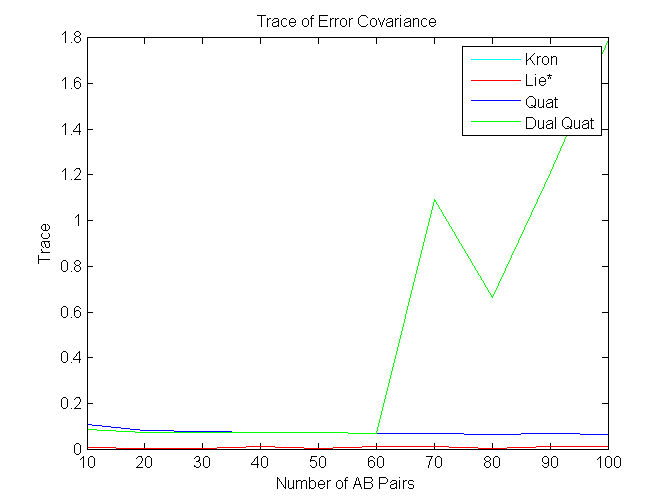
\includegraphics[scale=0.5]{figure/traceCov}
%\centering
%\label{fig:Trace}
%\caption{Trace of the Error Covariance Matrix}
%\end{figure}
The error covariance matrix $^e\Sigma$ can provide information about the variances of the independent and correlated error on each basis of Lie algebra. 
\end{comment}

\begin{comment}
\subsection{$\{A_{i}, B_{i}\}$ Pairs Generation}
There are various ways of generating noisy $\{A_{i},B_{i}\}$ pairs and different data sets can cause certain methods to perform badly or even to crash. To simulate different $AX=XB$ solvers with synchronous noisy $\{A_{i},B_{i}\}$ pairs, we first generate $B_{i}$ by randomly sampling the Lie algebra of matrix $B_{i}$, and then recover $B_{i}$ using the matrix exponential as shown below:
\begin{equation}
B_{i} = \exp \left(
\begin{array}{ccc}
\Omega_{i}  & & {\bf v_{i}}  \\ \\
{\bf 0}^T & & 0 \end{array}
\right).
\end{equation} 
Next, the noisy $A_{i}$ is obtained by $A_{i}= ^1\hspace{-0.05in}X_{i}\,\,B_i\,\,^2X_{i}^{-1}$ where $^1X_{i}$ and $^2X_{i}$ are calculated by applying small disturbances on the ground truth $X_{true}$: 
\begin{equation}
^mX_{i} = X_{true}\exp \left(
\begin{array}{ccc}
^m\Omega_{X_{i}}  & & ^m{\bf v}_{X_{i}}  \\ \\
{\bf 0}^T & & 0 \end{array}
\right)
\; \;
\text{where} \; \; m = 1,2
\label{X_disturb}
\end{equation}
where $\omega_{X_{i}}$ and ${\bf v}_{X_{i}}$ are drawn from independent Gaussian distributions. In order to test the sensitivity to different noise levels for each $AX=XB$ solver, we choose the mean of $\left(\omega_{X_{i}}^{T}, {\bf v}_{X_{i}}^{T}\right)^{T}$ to be ${\bf 0}_{6 \times 1}$ and its covariance matrix to be $\Sigma_{X_{i}} = \sigma^{2} \mathbb{I}_{6}$ with $\sigma$ ranging from 0 to 0.1.
\end{comment}

\begin{comment}
%-------------------------------------------------
\section{NUMERICAL SIMULATION}
In this section, we numerically simulated the Lie group method, the Kronecker product method, the quaternion method, and the dual quaternion method in Matlab  to compare the errors in both $R_{X}$ and $t_{x}$ with respect to different noise levels on $\{A_{i}, B_{i}\}$. 

The numerical simulation results are presented in Fig.\ref{roterror}, Fig.\ref{transerror}, and Fig.\ref{traceerror}. Figure \ref{roterror} shows that as the noise level $\sigma$ increases, Lie group method shows the least increase in rotation error, while the dual quaternion method's increase in the rotation error is the largest. The rotation errors of the Kronecker method (light blue line) and the quaternion method (dark blue line) are pretty close and they are even closer in terms of translational error (figure \ref{transerror}).
\end{comment}

\begin{comment}
\begin{figure}[h]
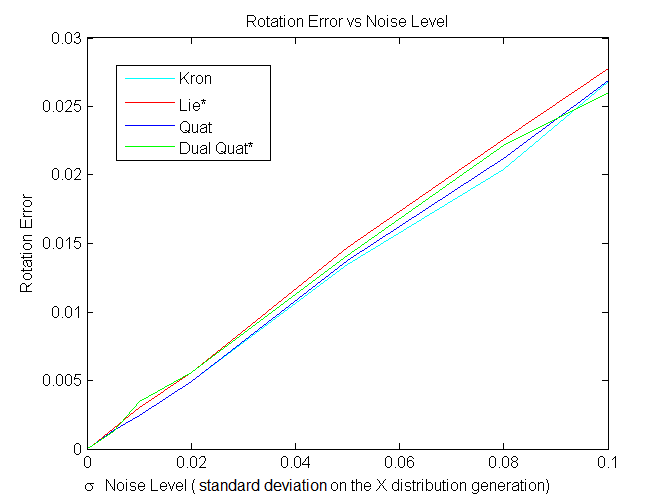
\includegraphics[width=3.3in]{figure/rotErrorRand}
\centering
\caption{Rotation Error v.s. Noise Level using Lie algebra Error Metric }
\label{roterror}
\end{figure}

{\color{blue} Lie$^{\star}$ is an improved version of the original Lie group method where ill-conditioned $\{A_{i},B_{i}\}$ pairs are eliminated to solve for the estimated $X$. This is due to the limitation of algorithm that $A_{i}$ or $B_{i}$ whose trace is equal or very close to -1 will cause the singularity of numerical computation. Different ways of generating $\{A_{i},B_{i}\}$ can affect the number of filtered pairs and certain ways can render the Lie group method giving $R_{X}$ with $\det(R_{X}) = -1$.\\

Dual Quat$^{\star}$ is an improved version of the original dual quaternion method which also eliminates certain $\{A_{i},B_{i}\}$ pairs by putting a boundary on the scalar parts of the dual quaternions of $A_{i}$ and $B_{i}$. Similar to the Lie group method, the way of generating $\{A_{i},B_{i}\}$ pairs can affect the number of filtered data, and this will affect the accuracy of the estimated $X$. In addition, certain ways of generating the data pairs can cause the dual quaternion method to give an invalid result from the filtered data. This problem can be solved by extracting a smaller portion of the given $\{A_{i},B_{i}\}$ pairs, but this also can degrade the accuracy of the result.  
\begin{figure}[h]
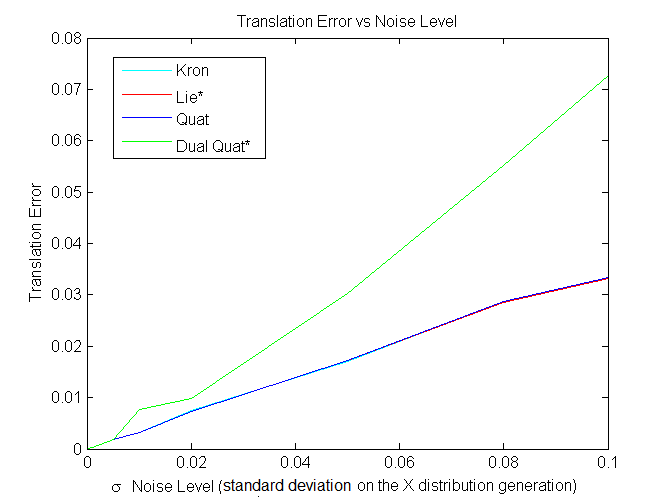
\includegraphics[width=3.3in]{figure/tranErrorRand}
\centering
\caption{Translation Error with Randomly Generated AB Pairs (with the improved Lie and Dual Quaternion methods)}
\label{transerror}
\end{figure}

\begin{figure}[h]
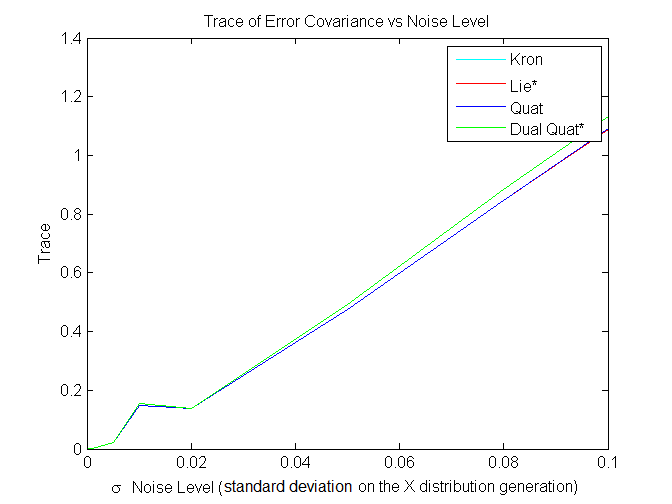
\includegraphics[width=3.3in]{figure/traceCovRand}
\centering
\caption{Trace of the Error Covariance Matrix}
\label{traceerror}
\end{figure}

In general, all of the traditional methods work well with near random Gaussian distributed noisy $\{A_{i},B_{i}\}$ pairs. However, it should be noted that in many applications, the information of $\{A_{i},B_{i}\}$ is obtained by moving the calibration sensor along a trajectory. Depending on the specifics of the trajectory as well as on the sample rate along the trajectory, the data may become ill conditioned for these methods.}
\end{comment}

%\begin{equation}
%\Sigma_{M_B}^3 =  (\widehat{-R^T_X t_x}) R^T_X \Sigma_{M_A}^1 R_X  +  R^T_X \Sigma_{M_A}^3 R_X
%\end{equation}
%\begin{align}
%\Sigma_{M_B}^4 &= -(\widehat{R^T_X t_x}) R^T_X \Sigma_{M_A}^1 R_X -(\widehat{R^T_X t_x})^T +  R^T_X \Sigma_{M_A}^3 R_X \nonumber \\
%&-(\widehat{R^T_X t_x})^T +  (\widehat{-R^T_X t_x}) R^T_X \Sigma_{M_A}^2 R_X + R^T_X \Sigma_{M_A}^4 R_X
%\end{align}



\begin{comment}
\subsection{Identities of Means and Covariances of Pdfs on SE(3)}
In this section we will prove two identities related to the mean and covariance of probability distributions on $SE(3)$ that will become useful to expand elements of the previously presented batch method.

\begin{theorem} \label{thm1}
If $M$ and $\Sigma$ are respectively the mean and covariance of $f(H)$, then
$M^{-1}$ and $Ad(M) \Sigma Ad^T(M)$ are respectively the mean and covariance of $f(H^{-1})$.
\end{theorem}

\begin{proof}
Let $f'(H) = f(H^{-1})$, and then $M'$ and $\Sigma'$ are the mean and covariance of $f'(H)$ satisfying the defining equations:
\begin{equation}
\begin{split}
&\int_{SE(3)} \log({M'}^{-1} H) f'(H) dH = \mathbb{O} \\
&\Sigma' = \int_{SE(3)} \log^{\vee}({M'}^{-1} H) [\log^{\vee}({M'}^{-1} H)]^{T}  f'(H) dH. 
\end{split}
\label{fprime}
\end{equation}
The first of Eq.(\ref{fprime})  can be rewritten as:
\begin{equation}
\int_{SE(3)} \log({M'}^{-1} H) f(H^{-1}) dH = \mathbb{O}
\label{f_prime_mean}
\end{equation}
By changing the variable $K = H^{-1}$ and using the invariance of integration under inversion (as described in the Appendix), Eq.(\ref{f_prime_mean}) can be written as:
$$ \int_{SE(3)} \log({M'}^{-1} K^{-1}) f(K) dK = \mathbb{O}. $$
Multiplying this equation on the left by $M'$ and on the right by ${M'}^{-1}$, and using the general property that
$$ H_1 (\log H_2) H_1^{-1} = \log (H_1 H_2 H_1^{-1}), $$
we get 
$$ \int_{SE(3)} \log(K^{-1} {M'}^{-1}) f(K) dK = \mathbb{O} $$
which is equivalent to 
$$ \int_{SE(3)} \log(({M'} K)^{-1} ) f(K) dK = \mathbb{O}. $$
But since
$$ \log (H^{-1}) = -\log H, $$
this means that
$$ \int_{SE(3)} \log( {M'} K) f(K) dK = \mathbb{O}, $$
and from the definition of mean, it must be that $M' = M^{-1}$.\\
Similarly, 
$$ \Sigma' = \int_{SE(3)} \log^{\vee}({M'}^{-1} H) [\log^{\vee}({M'}^{-1} H)]^{T}  f(H^{-1}) dH $$
which, under change of variables and substitution of $M' = M^{-1}$, becomes
$$ \Sigma' = \int_{SE(3)} \log^{\vee}(M K^{-1}) [\log^{\vee}(M K^{-1})]^{T}  f(K) dK. $$
But since by definition 
$$ Ad(H_1) \log^{\vee}(H_2) = \log^{\vee} (H_1 H_2 H_1^{-1}), $$
$$ Ad(M^{-1}) \Sigma' Ad^T(M^{-1}) = $$
$$ \int_{SE(3)} \log^{\vee}(K^{-1} M) [\log^{\vee}(K^{-1} M)]^{T}  f(K) dK .$$
Using $\log^{\vee}(K^{-1} M) = - \log^{\vee}(M^{-1} K)$ then gives
$$ Ad(M^{-1}) \Sigma' Ad^T(M^{-1}) = \Sigma $$
which, after inversion of the Ad matrices, completes the proof.
\end{proof}

It is also interesting to note that if $A_i X = X B_i$, then $(A_i X)^{-1} = (X B_i)^{-1}$ and rearranging gives 
$A_{i}^{-1} X = X B_{i}^{-1}$. This means that if we wish to, we can double the size of
the sets $A = \{A_i\}$ and $B=\{B_j\}$ by including the inverses of each entry in these sets. The consequence of this along with the fact that 
$$ f_{A^{-1}}(H) = f_A(H^{-1}) $$ 
provides a pdf describing incoming data of the form:
$$ \tilde{f}_A(H) \doteq \half (f_A(H) + f_A(H^{-1})) $$
and similar pdf can be obtained for $B$. These pdfs are ``symmetric functions'' in the sense that
$$ \tilde{f}_A(H) = \tilde{f}_A(H^{-1}) $$
and this has consequences that can be useful, as described in the following theorem.

\begin{theorem}
\label{thm2}
If $f_B(H) \in (L^1 \cap L^2)(SE(3))$ is a symmetric function and $K \in SE(3)$ and $f_X \in (L^1 \cap L^2)(SE(3))$ are arbitrary, then: \\
(a) $f_B(H)$ has its mean at the identity \\
(b)  $(f_X * f_B* f_{X^{-1}})(H)$ has its mean at the identity \\
(c) $f_B(K^{-1} H K)$ has its mean at the identity.
\end{theorem}

\begin{proof}
(a) By definition of mean on $SE(3)$,
$$ \int_{SE(3)} \log (M_B^{-1} H) f_B(H) dH = \mathbb{O} $$
and so
$$ \int_{SE(3)} \log (M_B^{-1} H) f_B(H^{-1}) dH = \mathbb{O}.$$
Let $K = H^{-1}$, and use the same operations as in Theorem \ref{thm1}, we arrive at
$$ \int_{SE(3)} \log (M_B K) f_B(K) dK = \mathbb{O}, $$
indicating that if $M_B$ is unique, then $M_B = M_B^{-1}$ and so $M_B = \mathbb{I}$.
Uniqueness can be guaranteed if $\Sigma$ is sufficiently small, which in turn can be guaranteed in our application if all samples $\{A_i\}$ and $\{B_j\}$ are replaced
by fractional powers $\{A_i^{1/n}\}$ and $\{B_j^{1/n}\}$.

(b) By definition, $M$, the mean of $(f_X * f_B* f_{X^{-1}})(H)$ must satisfy
$$ \int_{SE(3)} \log (M^{-1} H) (f_X * f_B* f_{X^{-1}})(H) dH = \mathbb{O}. $$
By showing that $(f_X * f_B* f_{X^{-1}})(H)$ is symmetric, the fact that $M = \mathbb{I}$ will follow from (a).
Using the definition of the convolution integral given in the Appendix, and expanding out both convolutions, we have:
\begin{equation}
\begin{split}
& (f_X * f_B* f_{X^{-1}})(H)\\
= &\int_{SE(3)} \int_{SE(3)}
f_X(J) f_B(J^{-1} K) f_{X^{-1}}(K^{-1} H) dJ dK
\\
= &\int_{SE(3)} \int_{SE(3)} f_{X^{-1}}(J^{-1}) f_B(K^{-1} J) f_{X}(H^{-1} K) dJ dK
\end{split}
\end{equation}
Here we have used the fact that $f_B$ is symmetric. By the same logic,
\begin{eqnarray*}
&& (f_X * f_B* f_{X^{-1}})(H^{-1}) = \\
&& \int_{SE(3)} \int_{SE(3)}
f_X(J') f_B(J'^{-1} K') f_{X^{-1}}(K'^{-1} H^{-1}) dJ' dK'
\end{eqnarray*}
We have the freedom to define $J'=H^{-1} K$ and $J^{-1} = K'^{-1} H^{-1}$.
The proposition will then be true if the remaining term,
$K^{-1} J = J'^{-1} K'$, holds. Indeed,
$$ J'^{-1} K' = (H^{-1} K)^{-1} H^{-1} J = K^{-1} J, $$
completes the proof of (b). Finally, (c) follows from (b) by letting $f_X(H) = \delta_K(H)$.
\end{proof}


\subsection{Batch Method Results}
To verify that this solution method produces a useful $X$, we used a numerical approach to simulate the $AX=XB$ problem by generating simulated $A$ and $B$ data streams. As is commonly done in the literature, and previously discussed in section \ref{qianli-numerical}, we generate the $\{B_{i}\}$ by randomly sampling each of the elements of the Lie algebra from a gaussian distribution of set mean and variance, and then matrix $B_{i}$ is recovered using matrix exponential. We then generate the noisy $A_{i}$ by $A_{i}= ^1\hspace{-0.05in}X_{i}\,\,B_i\,\,^2X_{i}^{-1}$ where $^1X_{i}$ and $^2X_{i}$ are given by exerting small disturbances on the same known $X_{true}$.

In Fig.\ref{normerror} and Fig.\ref{normerrorsym}, we show the performance of the Batch Method on simulated data. It should be noted that for case with the symmetrized data, the correct batch method solution, from the set of 4 possibilities (given (\ref{RQ})) can no longer be found by applying the cylinder constraints (as previously discussed). This is due to the fact that $M_A=M_B=\mathbb{I}$ for symmetrized data. However, we can still choose the correct $X$ by selecting one among the four candidates which minimizes the previously described objective function, $\| {\bf n}_{M_A}-R_X {\bf n}_{M_B} \|+w \| {\bf v}_{M_A} - \theta_{M_B} \widehat{\,{\bf t}_X} R_X {\bf n}_{M_B} + R_X {\bf v}_{M_B} \|$, by using the non-symmetrized data. The metric used for both cases is the relative normed error between the calculated solution $X_{calc}$ and the true solution $X_{true}$:

$$
E_{X} = \frac{\|X_{calc}-X_{true}\|}{\|X_{true}\|}.
$$  

\begin{figure}[h]
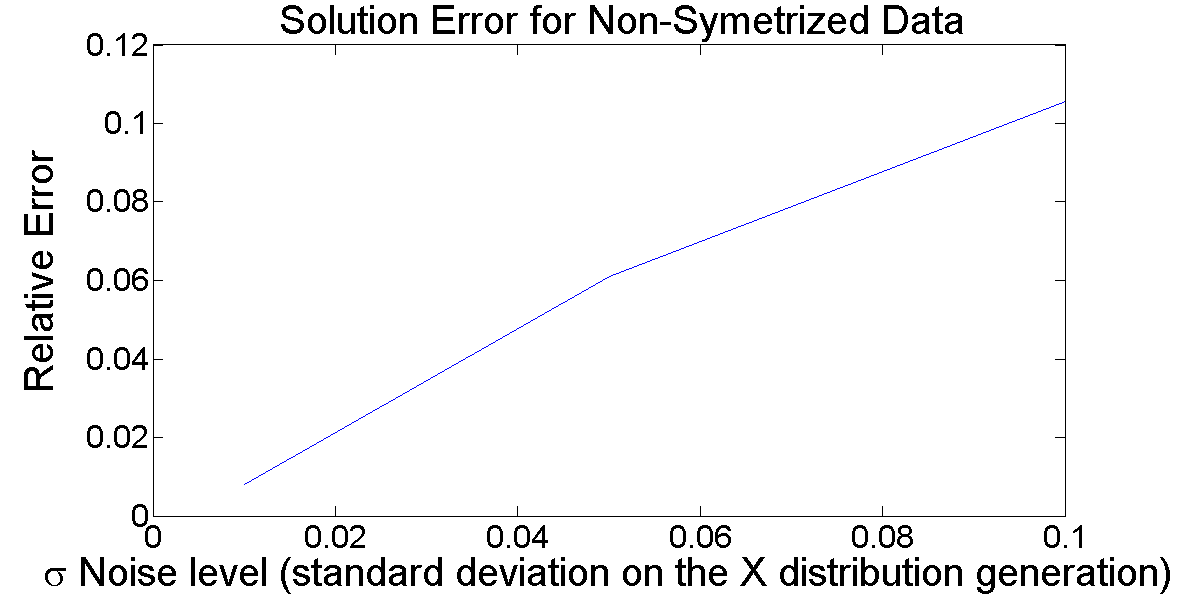
\includegraphics[width=3.3in]{figure/normerror}
\centering
\caption{Performance of the Batch Method at Various Noise Levels}
\label{normerror}
\end{figure}

\begin{figure}[h]
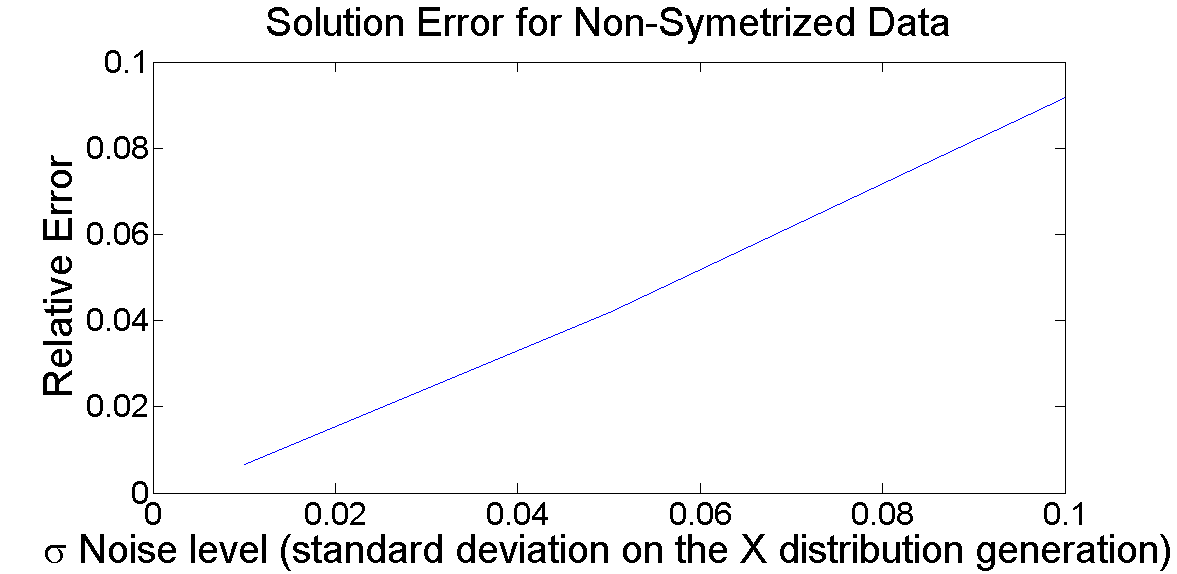
\includegraphics[width=3.3in]{figure/normerrorsym}
\centering
\caption{Performance of the Batch Method at Various Noise Levels for Symmeterized Data}
\label{normerrorsym}
\end{figure}

It is observed that symmetrized data provides, to a degree, a better solution of $X$. Additionally, symmetrizing the data provides more $\{A, B\}$ pairs, which will become important for methods described in the following sections.

\section{THE EXPANDED BATCH METHOD (THE CASE OF NOISY A's)} \label{batchnoise}

When the sensor that generates $B=\{B_j\}$ is accurate and there is significant
measurement noise in the set $A = \{A_i\}$, a single $X$ will not solve every instance of Eq.(\ref{main}) and hence the delta function in Eq.(\ref{mainconvall}) 
will not solve the problem. Instead, we seek a distribution $f_X(H)$ with (a priori unknown) mean $M_X$ and covariance $\Sigma_X$.

We can re-write Eq.(\ref{main}) as
\begin{equation} A_i = X B_i X^{-1} \label{main2} \end{equation}
and in a similar fashion as in Eq.(\ref{mainconvall}),we can write the probabilistic form of Eq.(\ref{mainconvall}) as
\begin{equation} f_A(H) = (f_X * f_B* f_{X^{-1}})(H). \label{mainconvallwnoise2} \end{equation}

In the subsections that follow, we derive the conditions on the mean and covariance of $f_X$ and
develop numerical methods for solving for these quantities.

\subsection{Conditions on $M_X$ and $\Sigma_X$}
Using the associativity of convolution, $f_X * f_B* f_{X^{-1}} = f_X * (f_B* f_{X^{-1}})$, 
and applying Eq.(\ref{meancovconvdef}) to Eq.(\ref{mainconvallwnoise2}) twice, we get
\begin{equation}
\boxed{\,
M_A = M_X \, M_B \, M_{X^{-1}}
\,}
\label{covprop2} \end{equation}
and
\begin{equation}
\begin{split}
\Sigma_{A} = Ad(M_{X})[Ad(M_{B^{-1}}) \Sigma_{X} Ad^T(M_{B^{-1}}) + \Sigma_{B}]Ad^T(M_{X})\\
+ \Sigma_{X^{-1}}.
\end{split}
\label{covprop22}
\end{equation}
Note that Eq.(\ref{covprop2}) and Eq.(\ref{covprop22}) are built on the use of (\ref{meancovconvdef}) twice so that they are approximations, unlike
Eq.(\ref{mainmain11}) and Eq.(\ref{mainmain12}) which are exact (by Theorem \ref{exactthm}). 
We can simplify this relationship in Eq.(\ref{covprop22}) by proving two identities related to the mean and 
covariance of probability distributions on $SE(3)$ given below.

As in the noise-free case, $(M_A,\Sigma_A)$ and $(M_B,\Sigma_B)$ are known from the data and are computed from
Eq.(\ref{datameancovconvdef}). The only difference is that now we seek $(M_X, \Sigma_X)$ instead of just $X$.

With these two properties, as well as the fact that $[Ad(H)]^{-1}=Ad(H^{-1})$, we can write Eq.(\ref{covprop22}) as:
\begin{flalign*}
\Sigma_A = &Ad(M_X) \, Ad(M_B^{-1}) \, \Sigma_{X} \, Ad^T(M_B^{-1}) \, Ad^T(M_X)\\
&+ Ad(M_X) \, \Sigma_{B} \, Ad^T(M_X) + Ad(M_X) \, \Sigma_{X}\, Ad^T(M_X), 
\end{flalign*}
or equivalently 
\begin{flalign*}
&Ad(M_X^{-1}) \, \Sigma_A \, Ad^T(M_X^{-1}) =\\
&Ad(M_B^{-1}) \, \Sigma_{X} \, Ad^T(M_B^{-1}) + \Sigma_{B} + \Sigma_{X}, 
\end{flalign*}
which leads to our final result 
\begin{equation}
\boxed{\,
\begin{split}
&\Sigma_{X} + Ad(M_B^{-1}) \, \Sigma_{X} \, Ad^T(M_B^{-1}) =\\
&Ad(M_X^{-1}) \, \Sigma_A \, Ad^T(M_X^{-1}) - \Sigma_{B}.
\end{split}
\,}
\label{covprop1112} \end{equation}
As in the noise-free case, $(A,\Sigma_A)$ and $(B,\Sigma_B)$ are known from the data and are computed from
Eq.(\ref{datameancovconvdef}). The only difference is that now we seek $(M_X, \Sigma_X)$ instead of just $X$.

\subsection{Computing $M_X$ and $\Sigma_X$}
From Eq.(\ref{covprop1112}), we can solve for $\Sigma_X$, given an $M_X$. This is done by taking the Kronecker product of both sides and writing
\begin{equation}
\begin{split}
[&Ad(M_B^{-1}) \otimes Ad(M_B^{-1}) + \mathbb{I}_{36}] {\rm vec}(\Sigma_X)\\
&= {\rm vec}(Ad(M_X^{-1}) \Sigma_{A} Ad^T(M_X^{-1}) - \Sigma_{B}),
\end{split}
\label{kroncovprop1112} \end{equation}
from which we obtain ${\rm vec}(\Sigma_X)$, and hence $\Sigma_X$.
Since $[Ad(M_B^{-1}) \otimes Ad(M_B^{-1}) + \mathbb{I}_6 \otimes  \mathbb{I}_6]$ in general will be non-singular, there is an exact solution of $\Sigma_X$ for every given $M_X$. This unique value of $\Sigma_X$ indicates the variation of $X$s, about the mean ($M_X$), needed to relate the sets of noisy data ($A$'s and $B$'s) in the $A_i=X_iB_iX_i^{-1}$ relationship. $\Sigma_X$ then becomes very useful for quantifying the``correctness" of a $M_X$. $\Sigma_{X_{calc}}$ is composed of the following variances on the values from the 6-dimensional Lie algebra,
\begin{equation}
\Sigma_{X_{calc}}=\left(
\begin{array}{cccccc}
\sigma_{\omega_1}^2 & \sigma_{\omega_1\omega_2} & \sigma_{\omega_1\omega_3} & \sigma_{\omega_1v_1} & \sigma_{\omega_1v_2} & \sigma_{\omega_1v_3}\\
\sigma_{\omega_2\omega_1} & \sigma_{\omega_2}^2 &\sigma_{\omega_2\omega_3} & \sigma_{\omega_2v_1} & \sigma_{\omega_2v_3} & \sigma_{\omega_2v_3}\\
\sigma_{\omega_3\omega_1} & \sigma_{\omega_3\omega_2} & \sigma_{\omega_3}^2 & \sigma_{\omega_3v_1} & \sigma_{\omega_3v_2} & \sigma_{\omega_3v_3}\\
\sigma_{v_1\omega_1} & \sigma_{v_1\omega_2} & \sigma_{v_1\omega_3} & \sigma_{v_1}^2 & \sigma_{v_1v_2} & \sigma_{v_1v_3}\\
\sigma_{v_2 \omega_1} & \sigma_{v_2 \omega_2} & \sigma_{v_2 \omega_3} & \sigma_{v_2 v_1} & \sigma_{v_2}^2 & \sigma_{v_2 v_3}\\
\sigma_{v_3 \omega_1} & \sigma_{v_3\omega_2} & \sigma_{v_3\omega_3} & \sigma_{v_3 v_1} & \sigma_{v_3 v_2} & \sigma_{v_3}^2\\
\end{array}\right).
\end{equation}
The information contained in $\Sigma_{X_{calc}}$ could be used to find the most favorable (least uncertainty in $X_{calc}$) directions for planning trajectories, sensor placement or other pose dependent tasks.

\subsection{Numerical Validation of $\Sigma_X$}
To verify that this formulation produced a meaningful $\Sigma_X$, we used a numerical approach that would allow us to, a prioir, know the true distribution of $X$. We simulate an $AX=XB$ calibration by generating simulated $A$ and $B$ data streams. The $B$s are chosen as poses along a trajectory in $SE(3)$. Since we must use relative motions, we generate $B^{ij}=B_i^{-1}B_{i+1}$ where $B_i$s are drawn from the two sample``s-shaped" trajectories on a sphere. After forming relative motions, $B_{ij}$'s, we calculate $A^{ij}= ^1\hspace{-0.05in}X_{ij}\,\,B_i\,\,^2X_{ij}^{-1}$, where $^1X_{ij}$ and $^2X_{ij}$ are drawn from a distribution with known mean ($X$) and covariance. Each calculation of $^kX_{ij}$ is tweaked as such:
\begin{equation} ^kX_{ij} \,\doteq\, X \,\, ^k\Delta_{ij} \label{noisybdef} \end{equation}
where $^k\Delta_{ij}$ is a matrix of small noises of the the form
$$ ^k\Delta_i \doteq
\exp \left(
\begin{array}{ccc}
\Omega (\delta t) & & {\bf v} (\delta t) \\ \\
{\bf 0}^T & & 0 \end{array}
\right) \,
\approx \, \mathbb{I}_4 + (\delta t) \left(
\begin{array}{ccc}
\Omega & & {\bf v} \\ \\
{\bf 0}^T & & 0 \end{array}
\right). $$
where $\Omega = - \Omega^T$ and ${\bf v}$ are random angular and translational velocities with components drawn independently from
a Gaussian distribution with variance $\sigma^2$, and $\delta t$ is a small finite time.

After calculating $\Sigma_X$ from Eq.($\ref{covprop1112}$), we can compare the calculated sample mean and covariance of $\{X_{ij}\}=\{^1X_{ij}\} \cup \{^2X_{ij}\}$ with the solved for values.


\begin{figure}[h]
\begin{center}
\setlength{\unitlength}{0.012500in}%
 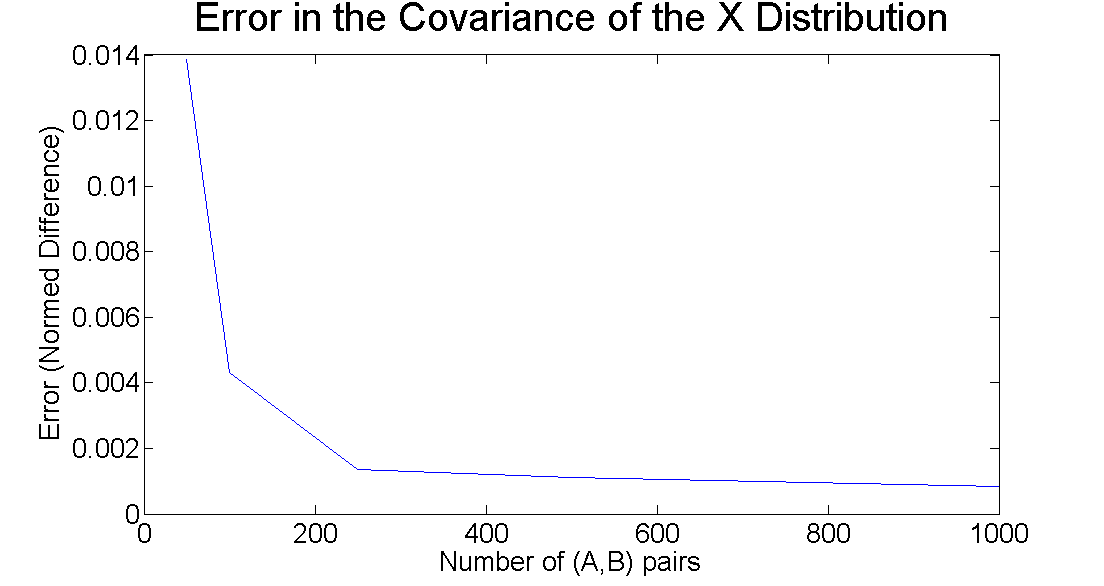
\includegraphics[width=3.3in]{figure/sigerror}
\end{center}
\caption{The Above Plot Shows that the $\Sigma_X$ is Calculated from ($\ref{covprop1112}$) and Becomes More Accurate as the Number of Data Samples Increases}
\label{figure_ASME} 
\end{figure}


\section{Relating the Covariances of a PDF and Its Symmetrized Version}

Recall that given an arbitrary pdf $f(H)$ with mean $M$ and covariance $\Sigma$, a symmetrized version is defined as:
$$ \tilde{f}(H) = \half ({f}(H) + {f}(H^{-1}) ). $$
Let $\tilde{M}$ and $\tilde{\Sigma}$ denote the mean and covariance of $\tilde{f}(H)$. 
Given that symmetrization of a pdf puts the mean of the result at the identity, we already know that $\tilde{M} = \mathbb{I}$.
The remaining question to ask is what the relationship is between the covariances of the original and symmetrized versions of a pdf.
This is answered here.

From the definition of covariance and the invariance of the integral over $SE(3)$ under inversions, and the fact that $\tilde{M} = \mathbb{I}$, the following equation
$$ \tilde{\Sigma} = \int_{SE(3)} \log^{\vee}(H)  [\log^{\vee}(H)]^T \tilde{f}(H) dH $$
can be simplified as:
$$ \tilde{\Sigma} = \int_{SE(3)} \log^{\vee}(H)  [\log^{\vee}(H)]^T {f}(H) dH. $$
This is not to be confused with
$$ {\Sigma} = \int_{SE(3)} \log^{\vee}(M^{-1} H)  [\log^{\vee}(M^{-1} H)]^T {f}(H) dH. $$
where
$$ \int_{SE(3)} \log^{\vee}(M^{-1} H)  {f}(H) dH = \mathbb{O}. $$

Though there appears to be no simple exact relationship between $\tilde{\Sigma}$ and ${\Sigma}$, in the case when $\|\Sigma\|$ and $\|M\|$ are both reasonably
small, an approximate relationship can be constructed by using the Baker-Campbell-Hausdorf formula to expand out $\log^{\vee}(M^{-1} H)$. 
This was done in \cite{wang06}, and the result (modulo different notation) is:
\begin{equation}
\tilde{\Sigma} = \Sigma + (\log^{\vee} M)(\log^{\vee} M)^T + \half \left(\Sigma \, ad^T(\log M) + ad(\log M) \, \Sigma\right)
\label{sigtildesig}
\end{equation}
If $(M,{\Sigma})$ is known a priori, then $\tilde{\Sigma}$ can be computed from them. Due to the simple computation of $\tilde{\Sigma}$, Eq.(\ref{sigtildesig}) can be used as a consistency
check on the accuracy of $M$ and $\Sigma$ by computing the norm of the difference of both sides.
\end{comment}


\section{CONCLUSION AND FUTURE DIRECTIONS}
\label{sec:conclusion}
In this paper, the ``AX=XB'' formulation of the sensor calibration problem is examined, which is widely used in camera calibration, humanoid head-eye calibration, robot eye-to-hand calibration, aerial vehicle sensor calibration, and IGT sensor calibration. A review of some of the most influential and effective methods was presented and their positive and negative traits were discussed. For the various $AX=XB$ solvers, the focus is put on the case where there is noise on the incoming sensor data, and therefore multiple sensor readings are needed. It was clear that each algorithm has strengths and weaknesses in different contexts, and it is important to use the appropriate method for different circumstances. %the circumstance.

In addition to measurement error contributing to noise, it was emphasized that the sensor data streams containing the $A$s and $B$s may be present at different sampling rates, may be asynchronous, and/or each stream may contain gaps in information. Therefore, a probabilistic method is reviewed in detail which is used for calculating the calibration transformation that works for data without any a priori knowledge of the correspondence between the $A$s and $B$s. Data selection is of critical importance to $AX=XB$ solvers. Depending on the quality of the data pairs, the usage of data selection techniques can either greatly improve the final result or prevent the solver from failing. 

Though many algorithms are available for hand-eye calibration, which algorithm is preferable for the given type and number of motions is still unclear. It will be helpful to categorize the type of motions and their corresponding preferable solvers.  


\begin{comment}
%%%%%%%%%%%%%%%%%%%%%%%%%%%%%%%%%%%%%%%%%%%%%%%%%%%%%%%%%%%%%%%%%%%%%%
\begin{acknowledgment}
The authors would like to recognize NSF Grant RI-Medium: IIS-1162095, which served to support this work. The authors would also like to acknowledge the support of M. Kendal Ackerman, Alexis Cheng and Emad M. Boctor, colleagues in this endeavor at Johns Hopkins University.

Chirikjian’s contribution to this material is based upon work supported by (while serving at) the National Science Foundation.
Any opinion, findings, and conclusions or recommendations expressed in this material are those of the author(s)
and do not necessarily reflect the views of the National Science Foundation.
\end{acknowledgment}
\end{comment}


%
%%%%%%%%%%%%%%%%%%%%%%%%%%%%%%%%%%%%%%%%%%%%%%%%%%%%%%%%%%%%%%%%%%%%%%%
\appendix       %%% starting appendix
\section*{Appendix A: Integration and Convolution on SE(3)}

This appendix reviews the features of integration and convolution on the group $SE(3)$ that are
relevant to the formulation in this paper. For more detailed treatments see \cite{myoldbook, vol2}.

\subsection*{Integration}

$SE(3)$ is a six-dimensional matrix Lie group. If $H = H({\bf q})$ where ${\bf q} = [q_1,....,q_6]^T$ is a global set of coordinates, then
functions $f:SE(3) \rightarrow \mathbb{R}$ can be integrated as
$$ \int_{SE(3)} f(H) dH \doteq \int_{{\bf q} \in D} f(H({\bf q})) |J({\bf q})| d{\bf q} $$
where $D$ is the domain of integration in the parameter space and $d{\bf q} = dq_1 dq_2 \cdots dq_6$. 
The Jacobian determinant $|J({\bf q})|$ is computed from the Jacobian matrix:
$$ J({\bf q}) = \left[\left(H^{-1} \frac{\partial H}{\partial q_1}\right)^{\vee}; \left(H^{-1} \frac{\partial H}{\partial q_2}\right)^{\vee};\,\cdots\,
\left(H^{-1} \frac{\partial H}{\partial q_6}\right)^{\vee}\right]. $$
For example, if Cartesian coordinates are used for the translation vector and $ZXZ$ Euler angles are used
for rotations, then ${\bf q} = [x,y,z,\alpha,\beta,\gamma]^T$, $D=\mathbb{R}\times\mathbb{R}\times\mathbb{R}\times[0,2\pi]\times[0,\pi]\times[0,2\pi]$ and $|J({\bf q})| = \sin \beta$. While $D$ and $J({\bf q})$ will change depending on which parametrization is used, the value of the integral itself does not as it is a property of the Lie group. The integral depends on the function themselves but not a matter of how the function is expressed or the coordinates of the integral.

$SE(3)$ is unimodular, which means that the integation measure, $dH = |J({\bf q})| d{\bf q}$, has the property that for any
fixed $H_0 \in SE(3)$ and ``well-behaved fuction\footnote{Here a well-behaved function means a function for which the integral exists, and hence
$f \in L^1(SE(3))$, and later that the convolution integral exists, which is guaranteed by further requiring that
$f \in L^2(SE(3))$. And so, with the notable exception of the Dirac delta function, the discussion is restricted to
$f \in (L^1 \cap L^2)(SE(3))$.}'' $f:SE(3) \rightarrow \mathbb{R}$, \cite{myoldbook}
\begin{equation}
\int_{SE(3)} f(H_0 \circ H) dH = \int_{SE(3)} f(H \circ H_0) dH = \int_{SE(3)} f(H) dH.
\label{defuni}
\end{equation}
In addition, it can be shown that when these conditions hold, so too does
\begin{equation}
\int_{SE(3)} f(H^{-1}) dH = \int_{SE(3)} f(H) dH.
\label{invdsdcf}
\end{equation}
A common source of confusion is that many books on Lie groups are concerned with compact Lie groups, which possess both bi-invariant metrics
and bi-invariant integration measures. When discussing the noncompact case, bi-invariant metrics generally do not exist (except for special cases
such as products of tori and Euclidean spaces), and they do not exist for $SE(3)$. Though bi-invariant integration measures also do not exist in general,
they do exist for a broader class of special noncompact Lie groups%than those that have bi-invariant metrics
, and this includes $SE(3)$. 

\subsection*{Convolution} \label{convsec}

Given two functions, $f_1, f_2 \in (L^1 \cap L^2)(SE(3))$, the convolution is defined as
\begin{equation}
(f_1 * f_2)(H) \doteq \int_{SE(3)} f_1(K) f_2(K^{-1} H) dK. 
\label{convdef}
\end{equation}
This integral can be rewitten in a number of equivalent forms using Eq.~(\ref{defuni}) and Eq.~(\ref{invdsdcf}).
Convolution inherits the associative property from the underlying group, which is written as 
$$ (f_1 * f_2) * f_3 = f_1 * (f_2 * f_3) $$
where the dependence of these functions on $H$ has been temporarily suppressed. Analogous with the way convolution inherits associativity, it 
also inherits noncommutativity for general functions, with the exception of special functions called ``class functions''.

The Dirac delta function on $SE(3)$ is defined as follows:
\begin{equation}\label{equ2}
\delta{(H)}=
\left\{
\begin{array}{ll}
+\infty, & H=I \\
0, & H \neq I
\end{array}
\right.
\end{equation}
which satisfies the constraint that: 
\begin{equation}\label{equ3}
\int_{SE(3)}\delta{(H)}dH=1.
\end{equation}
A slightly further expansion of allowable functions to include shifted delta functions of the form:
\begin{equation}
\delta_X(H) \doteq \delta(X^{-1} H) = \delta( H X^{-1}).
\end{equation}
The unshifted delta function is an example of a symmetric function, in that $\delta(H) = \delta(H^{-1})$.

If the class of functions is expanded to consider beyond $(L^1 \cap L^2)(SE(3))$
to include Dirac delta functions, then the following is true for every $f \in (L^1 \cap L^2)(SE(3))$:
$$ (f * \delta)(H) = (\delta * f)(H) = f(H). $$

Using the properties of the invariant integral on $SE(3)$, convolving a shifted delta function with an arbitrary
function transfers the shift:
\begin{equation}
\begin{split}
(\delta_X * f)(H) =& \int_{SE(3)} \delta(X^{-1} K) f(K^{-1} H) dK \\
=& \int_{SE(3)} \delta(J) f((XJ)^{-1} H) dK = f(X^{-1} H) \\
\end{split}
\end{equation}
where the change of variables $J = X^{-1} K$ and the invariance of integration have been used.

\begin{comment}
Similarly,
$$ (\delta_X * f * \delta_{X^{-1}})(H) = f(X^{-1} H X). $$
Using the associative property,
\begin{equation}
\begin{split}
&(\delta_X * f_1 * \delta_{X^{-1}}) * (\delta_X * f_2 * \delta_{X^{-1}}) \\
&= \delta_X * f_1 * (\delta_{X^{-1}} * \delta_X) * f_2 * \delta_{X^{-1}} \\ 
&= \delta_X * (f_1 * f_2)* \delta_{X^{-1}}. 
\end{split}
\end{equation}
\end{comment}

\begin{comment}
\subsection*{Symmetric Functions and Class Functions}

A symmetric function is one with the property that
$$ s(H) = s(H^{-1}). $$
There are several ways to construct symmetric pdfs from nonsymmetric ones. For example, if $f$ is a pdf, 
$\tilde{f}(H) = \half(f(H) + f(H^{-1})$ is symmetric (with the factor of $1/2$ necessary to make the result a pdf).
$f(H)\cdot f(H^{-1})/((f*f)(\mathbb{I}))$ is also symmetric and normalized to be a pdf (where $\cdot$ is just scalar
multiplication of functions). Also, if $f(H)$ is an arbitrary pdf and $f'(H) = f(H^{-1})$, then $(f*f')(H)$ will be symmetric.

Using the invariance properties of the integral over $SE(3)$, it is not difficult to see that 
\begin{eqnarray*}
(s_1 * s_2)(H) &=& \int_{SE(3)} s_1(K) s_2(K^{-1} H) dK \\
&=& \int_{SE(3)} s_1(K^{-1}) s_2(H^{-1} K) dK. \end{eqnarray*}
Then changing variables as $J = H^{-1} K$, $HJ =K$, and $K^{-1} = J^{-1} H^{-1}$ so
$$ (s_1 * s_2)(H) = \int_{SE(3)} s_2(J) s_1(J^{-1} H^{-1}) dJ = (s_2 * s_1)(H^{-1}). $$
This is not the same as saying that the convolution of two symmetric functions is symmetric. Nor does it say that
the convolution of symmetric functions is commutative. But, it does say that
the convolution of a symmetric function with itself is symmetric. 

In general, the only functions on a group that commute under convolution with every function are the class functions.
A class function has the property that
$$ \chi(K H K^{-1}) = \chi(H) $$
for every $H,K$ in the group. For example, $\delta$ is a class function for $SE(3)$, and the fact that it commutes under
convolution was already explained in (\ref{convsec}).
\end{comment}

% Here we show that in general class function commute under convolution.
%
%*** will fill if needed. may not be very relevant ***
%
%Unfortunately, no class functions on $SE(3)$ are in $(L^1 \cap L^2)(SE(3))$.


%%%%%%%%%%%%%%%%%%%%%%%%%%%%%%%%%%%%%%%%%%%%%%%%%%%%%%%%%%%%%%%%%%%%%%%
%\section*{Appendix B: Head of Second Appendix}
%\subsection*{Subsection head in appendix}
%The equation counter is not reset in an appendix and the numbers will
%follow one continual sequence from the beginning of the article to the very end as shown in the following example.
%\begin{equation}
%a = b + c.
%\end{equation}


%%%%%%%%%%%%%%%%%%%%%%%%%%%%%%%%%%%%%%%%%%%%%%%%%%%%%%%%%%%%%%%%%%%%%%
% The bibliography is stored in an external database file
% in the BibTeX format (file_name.bib).  The bibliography is
% created by the following command and it will appear in this
% position in the document. You may, of course, create your
% own bibliography by using thebibliography environment as in
%
% \begin{thebibliography}{12}
% ...
% \bibitem{itemreference} D. E. Knudsen.
% {\em 1966 World Bnus Almanac.}
% {Permafrost Press, Novosibirsk.}
% ...
% \end{thebibliography}

% Here's where you specify the bibliography style file.
% The full file name for the bibliography style file 
% used for an ASME paper is asmems4.bst.
\bibliographystyle{asmems4}

% Here's where you specify the bibliography database file.
% The full file name of the bibliography database for this
% article is asme2e.bib. The name for your database is up
% to you.
\bibliography{asme2e}
\end{document}